\chapter{Descriere funcțională și validare}
\label{chap:functionalitati}

\section{Prezentarea interfeței grafice}

Interfața BeeSmart este construită pentru un utilizator care lucrează în teren și are nevoie de acces rapid la informații. La prima pornire fără sesiune activă, aplicația afișează un ecran de splash cu animații de prezentare, după care trece automat la fluxul de autentificare. Odată autentificat, utilizatorul ajunge pe ecranul principal, de unde poate naviga către stupine, inspecții, task-uri, profil și alte funcționalități. Navigarea principală este realizată prin bara de navigație de jos, iar ecranele de creare sau editare se deschid ca fluxuri dedicate.

Designul folosește ecrane Compose structurate pe carduri, liste și formulare. Componentele reutilizabile \texttt{BeeSmartPanel} și \texttt{BeeSmartEmptyState} unifică aspectul tuturor ecranelor. Culorile semantice \texttt{StatusOk}, \texttt{StatusWatch} și \texttt{StatusDanger} comunică vizual nivelul de atenție necesar pentru un stup sau o operație. Fiecare zonă funcțională are stări clare: încărcare, succes, eroare sau stare goală. De exemplu, ecranul de statistici DeepBee afișează un mesaj dacă nu există încă analize AI pentru stupul curent, iar ecranul meteo afișează o stare indisponibilă dacă cheia OpenWeatherMap nu este configurată. Ecranul principal al aplicației este prezentat în figura~\ref{fig:home}.

\begin{figure}[H]
	\centering
	\subfigure[Salut și sumarul stupinei]{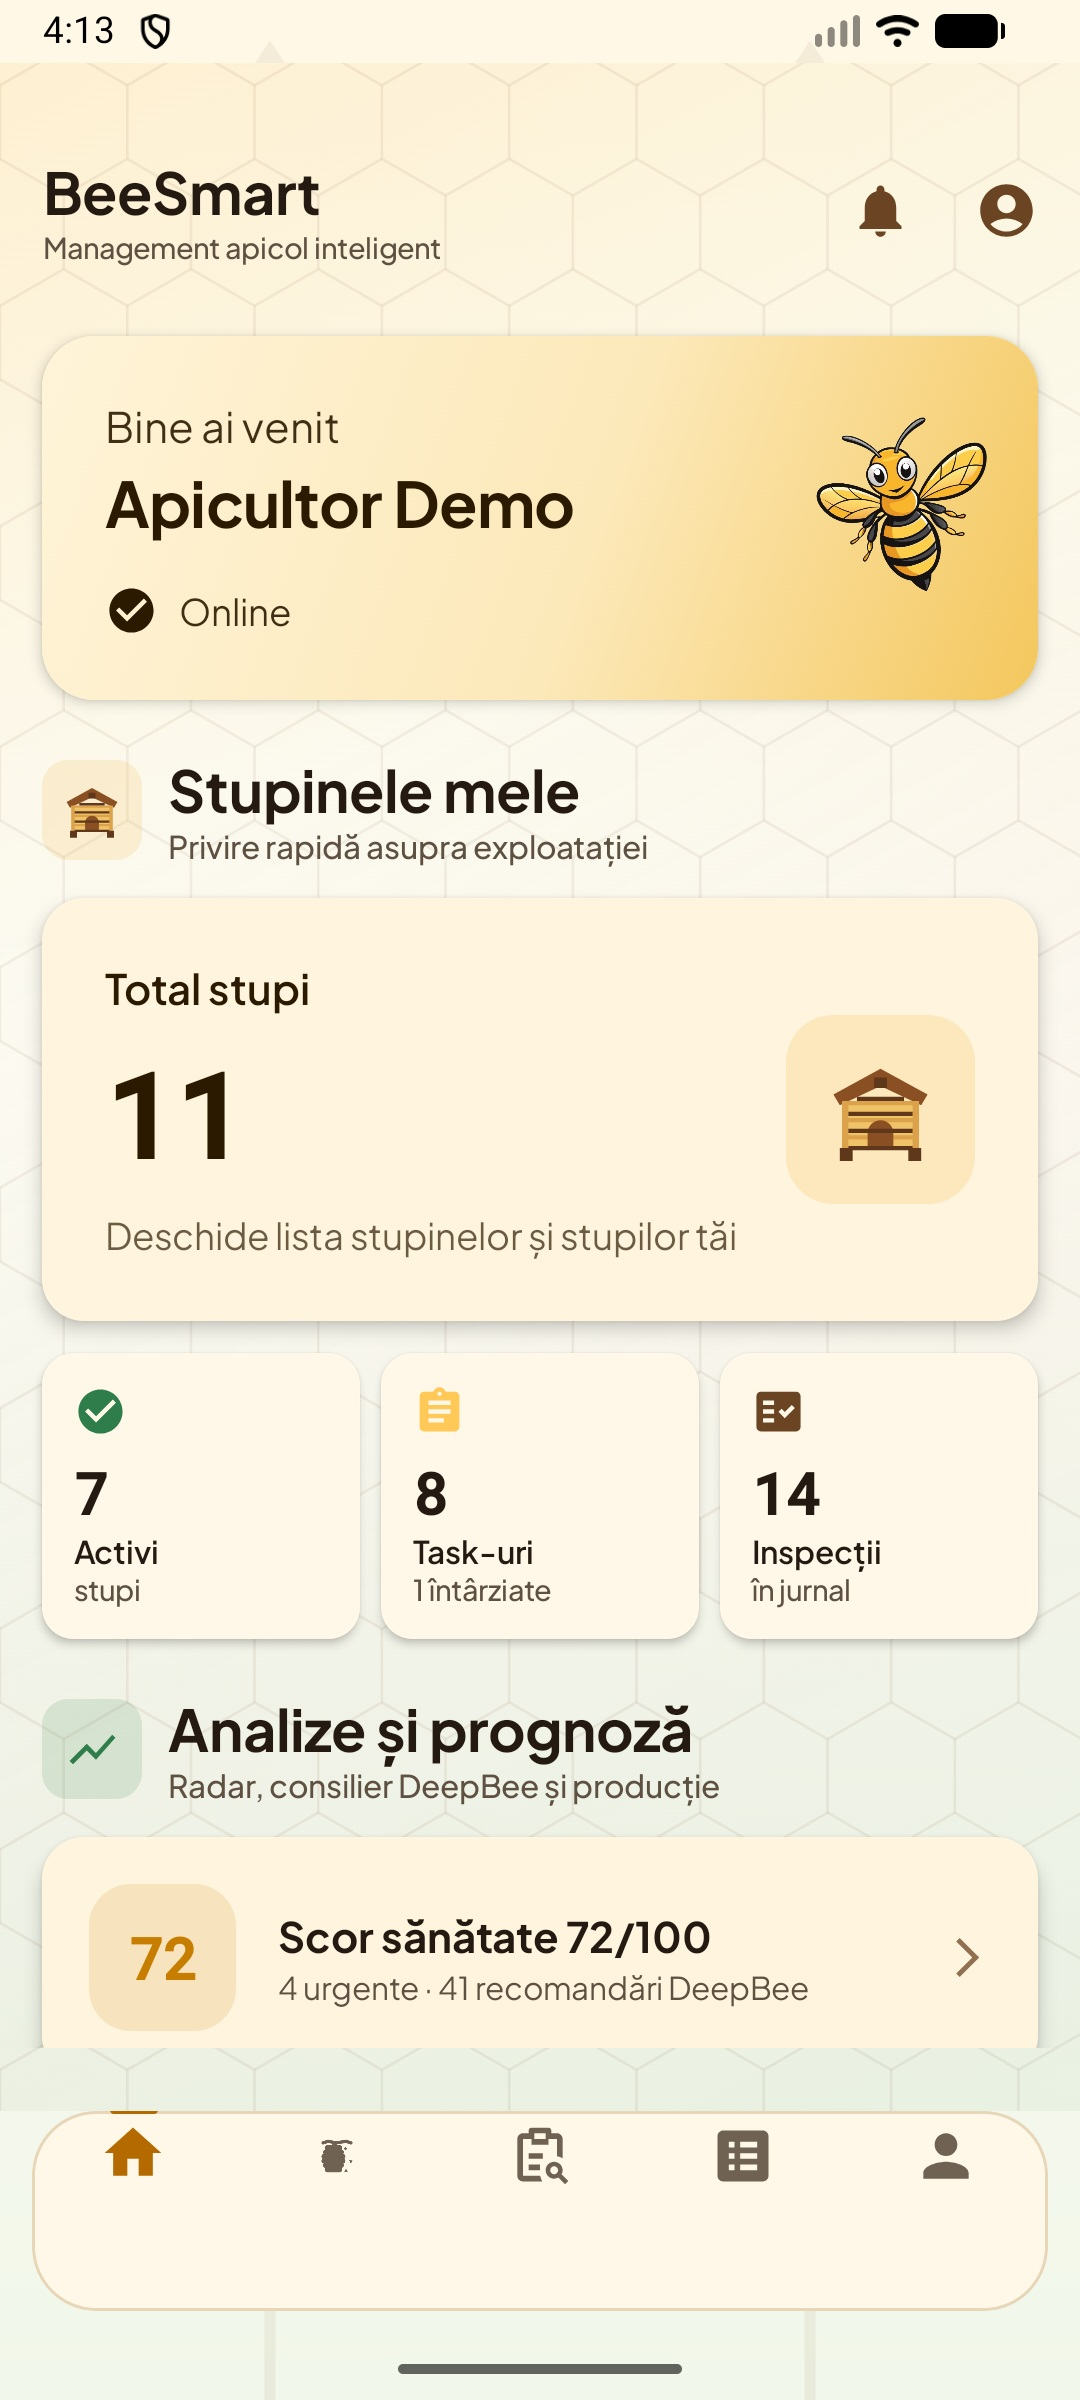
\includegraphics[width=0.40\textwidth]{./images/screenshots/04-dashboard-updated.jpg}}
	\hfill
	\subfigure[Acces rapid la module]{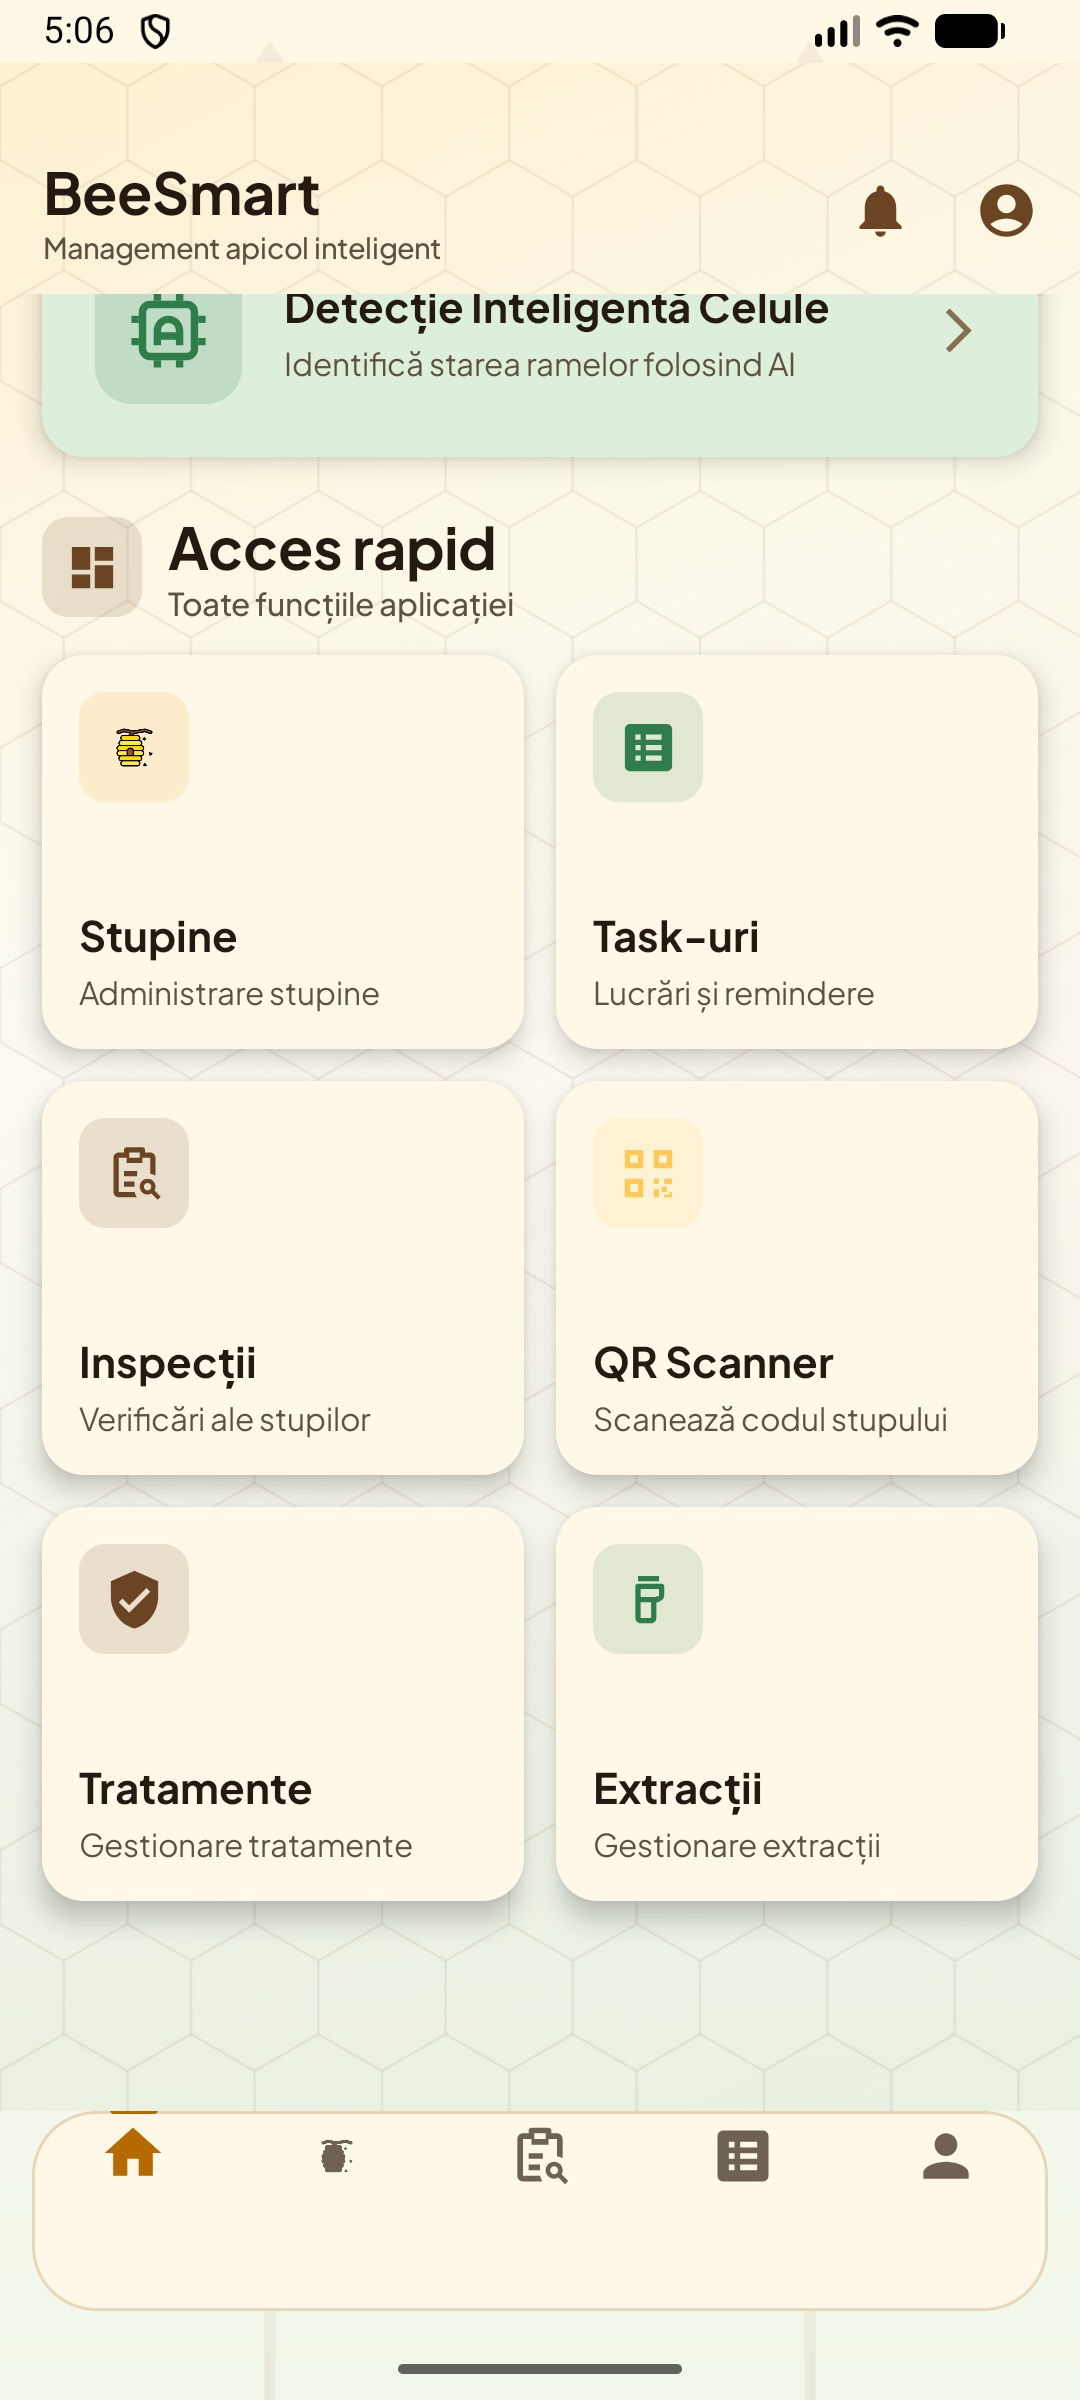
\includegraphics[width=0.40\textwidth]{./images/screenshots/home-modules-updated.jpg}}
	\caption{Ecranul principal al aplicației: partea de sumar a stupinei și zona de acces rapid la modulele de lucru.}
	\label{fig:home}
\end{figure}

\section{Scenariul de autentificare}

Primul scenariu este crearea unui cont și autentificarea. Utilizatorul accesează fluxul de register, introduce datele necesare, iar backend-ul creează contul, salvează parola hash-uită și generează token-urile necesare. În funcție de configurarea email, utilizatorul poate primi un link de confirmare. Linkul poate deschide aplicația prin schema \texttt{beesmart://confirm-email} sau prin domeniul \texttt{https://app.beesmart.ro/confirm-email}.

La login, aplicația primește un access token și un refresh token. Access token-ul este folosit pentru cererile protejate, iar refresh token-ul permite obținerea unui token nou fără reautentificare. \texttt{AuthInterceptor} tratează expirarea token-ului și reia cererea cu token-ul nou, atunci când refresh-ul reușește. Dacă refresh-ul eșuează, sesiunea este curățată și utilizatorul trebuie să se autentifice din nou. Ecranele de autentificare și de înregistrare sunt prezentate în figura~\ref{fig:auth}.

\begin{figure}[H]
	\centering
	\subfigure[Autentificare]{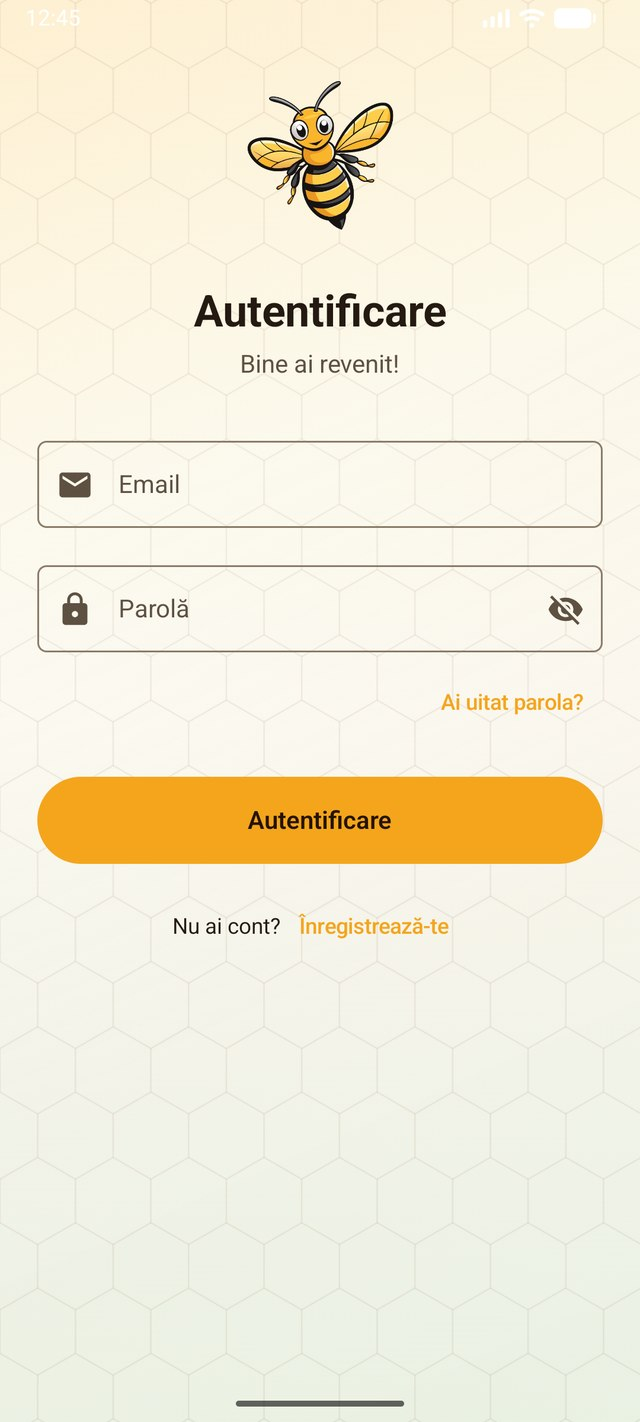
\includegraphics[width=0.40\textwidth]{./images/screenshots/01-login.jpg}}
	\hfill
	\subfigure[Înregistrare cont nou]{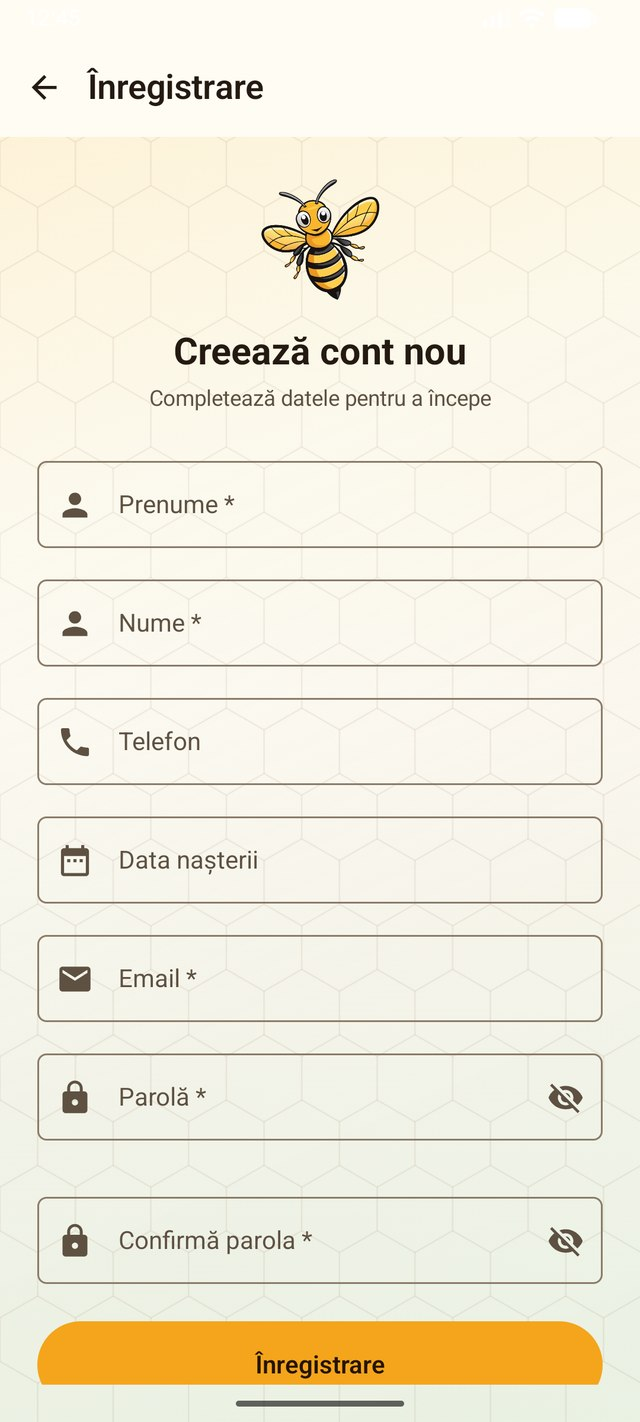
\includegraphics[width=0.40\textwidth]{./images/screenshots/02-register-empty.jpg}}
	\caption{Fluxul de autentificare: ecranul de login și formularul de înregistrare.}
	\label{fig:auth}
\end{figure}

\section{Crearea unei stupine}

După autentificare, utilizatorul poate crea o stupină. Formularul conține nume, descriere și locație. Locația este importantă nu doar ca informație descriptivă, ci și pentru integrarea meteo. \texttt{WeatherRepository} folosește textul locației pentru geocodare și apoi pentru obținerea datelor de vreme curentă.

Dacă utilizatorul creează stupina fără internet, aplicația generează un id local, salvează \texttt{ApiaryEntity} în Room și adaugă operația în \texttt{sync\_queue}. În listă, stupina apare imediat, chiar dacă serverul nu a confirmat-o încă. Când conexiunea revine, \texttt{SyncManager} trimite cererea către backend, primește id-ul de server și actualizează rândul local. Formularul de creare a unei stupine este ilustrat în figura~\ref{fig:create-apiary}.

\begin{figure}[H]
	\centering
	\subfigure[Formular gol]{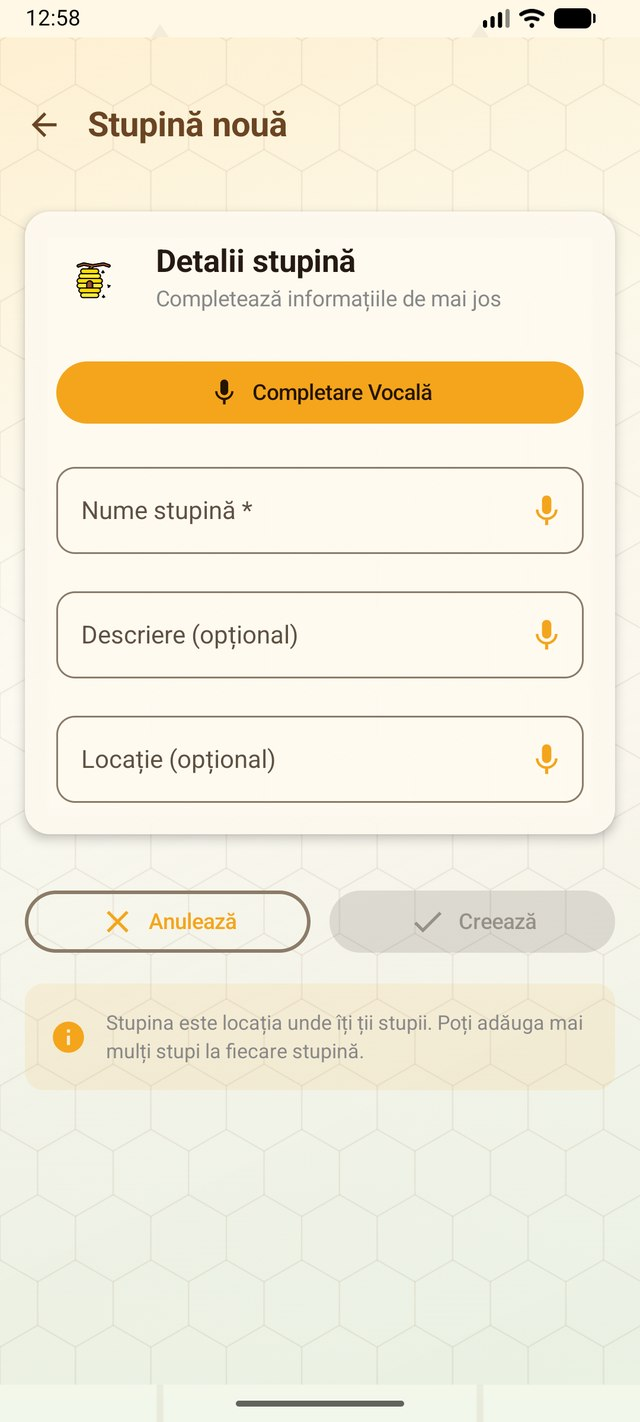
\includegraphics[width=0.40\textwidth]{./images/screenshots/06-create-apiary-form.jpg}}
	\hfill
	\subfigure[Formular completat]{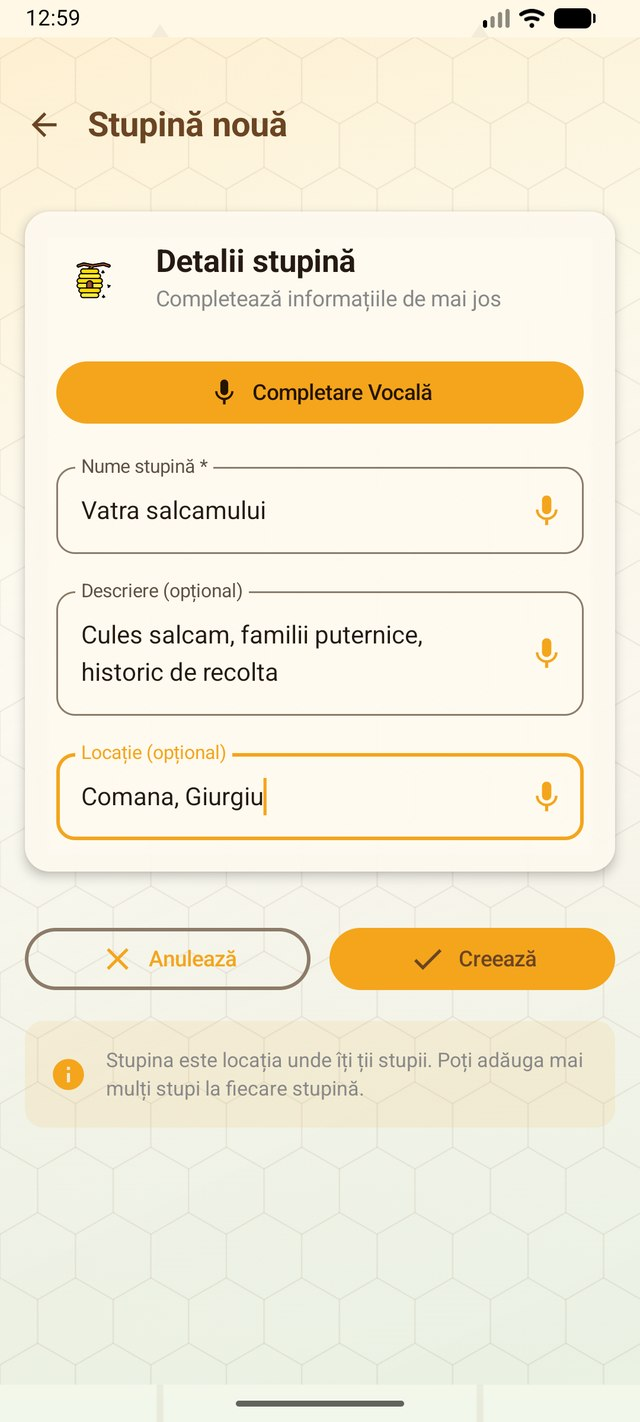
\includegraphics[width=0.40\textwidth]{./images/screenshots/07-create-apiary-filled.jpg}}
	\caption{Crearea unei stupine: formularul cu nume, descriere și locație, cu opțiunea de completare vocală.}
	\label{fig:create-apiary}
\end{figure}

\section{Adăugarea și gestionarea stupilor}

În interiorul unei stupine, utilizatorul poate adăuga stupi. Modelul \texttt{Hive} conține câmpuri precum nume, tip, status, note, prezența mătcii, vârsta mătcii, rame cu albine, rame cu puiet, rame cu miere și ultima inspecție. Aceste câmpuri permit o descriere rapidă a stării generale a stupului, fără a intra neapărat în istoricul complet al inspecțiilor.

Stupii pot fi creați și offline. Dacă stupina părinte nu a fost încă sincronizată, \texttt{SyncManager} amână crearea stupului până când stupina primește \texttt{serverId}. Această logică este importantă deoarece backend-ul cere id-ul real al stupinei pentru ruta de creare a stupului.

Fiecare stup poate avea un cod QR generat din linkul de deep link. Codul poate fi salvat ca imagine, distribuit sau exportat într-un PDF simplu. În teren, scanarea codului QR permite deschiderea rapidă a fișei stupului, fără căutare manuală în listă. Lista stupilor, formularul de adăugare și codul QR generat sunt prezentate în figura~\ref{fig:hives}.

\begin{figure}[H]
	\centering
	\subfigure[Lista stupilor cu statusuri]{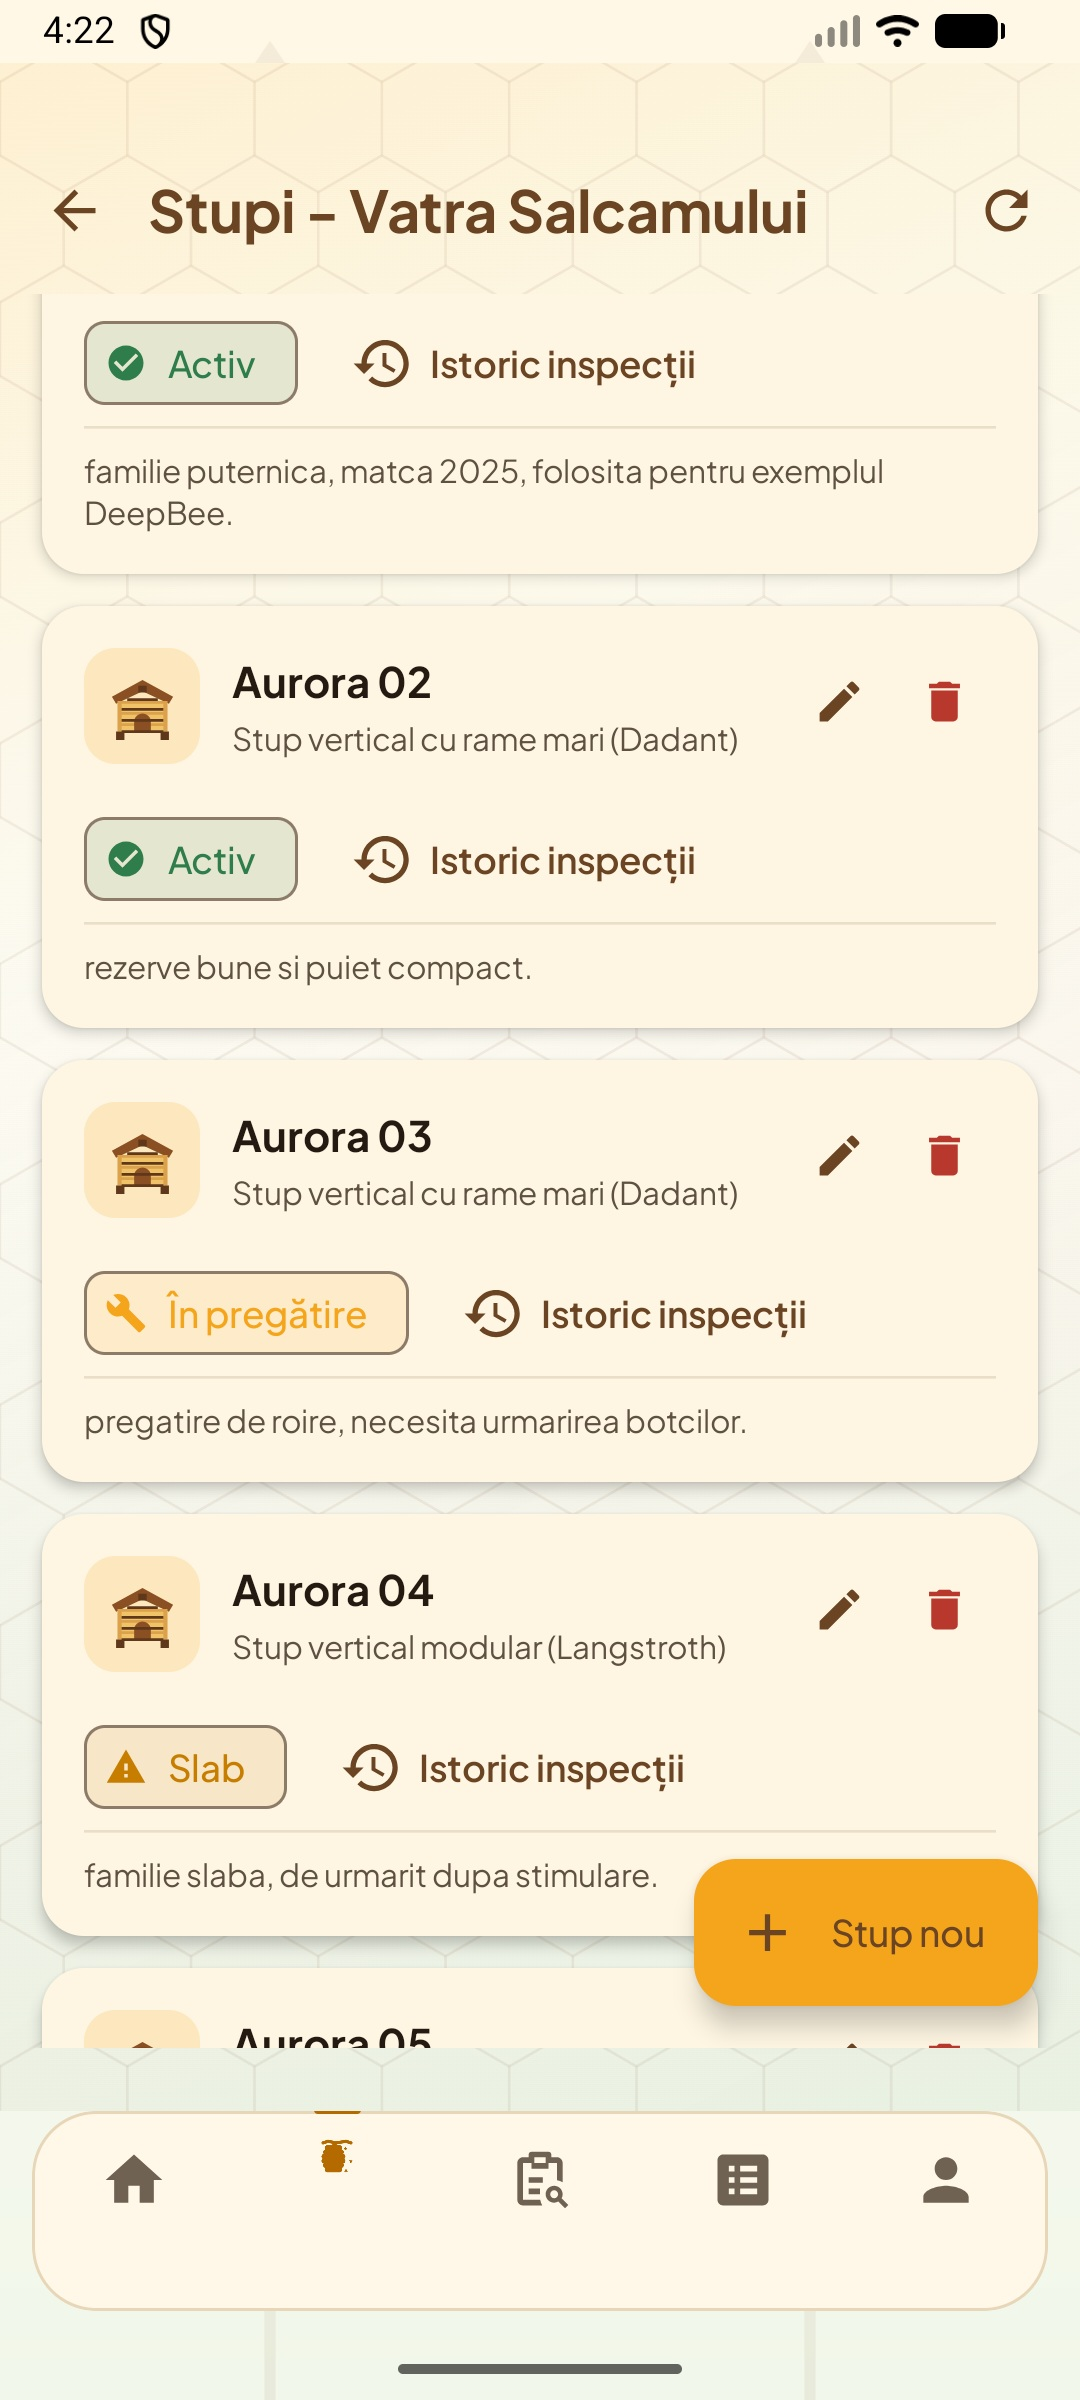
\includegraphics[width=0.30\textwidth]{./images/screenshots/16-vatra-hives-risk-list-updated.jpg}}
	\hfill
	\subfigure[Formular de adăugare stup]{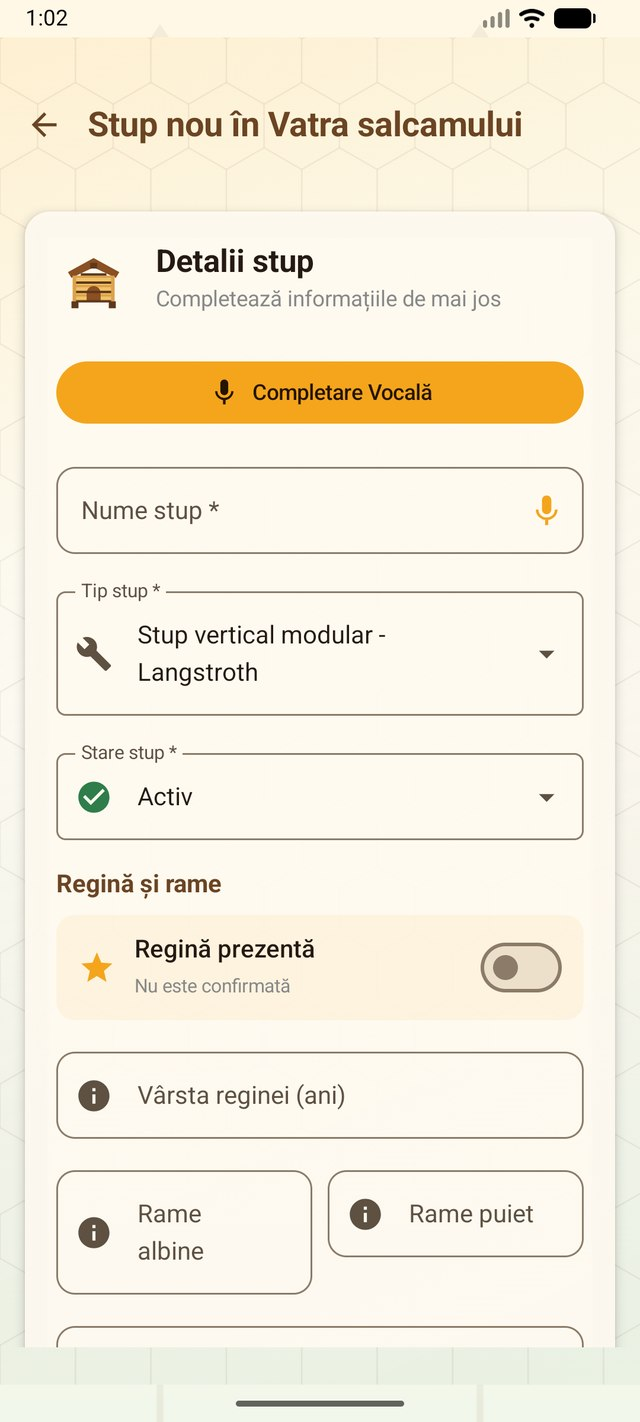
\includegraphics[width=0.30\textwidth]{./images/screenshots/10-create-hive-form.jpg}}
	\hfill
	\subfigure[Cod QR al stupului]{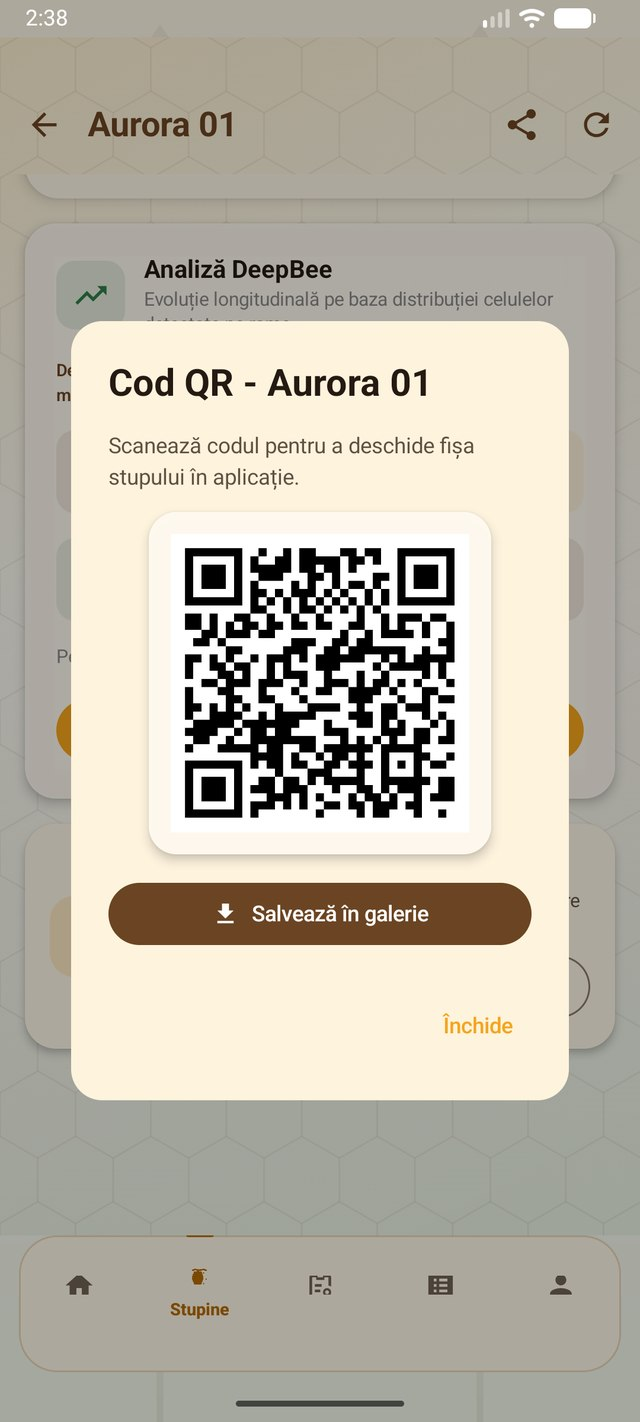
\includegraphics[width=0.30\textwidth]{./images/screenshots/hive-qr.jpg}}
	\caption{Gestionarea stupilor: lista cu statusuri (activ, slab, fără regină), formularul de creare și codul QR generat pentru deschiderea rapidă a fișei.}
	\label{fig:hives}
\end{figure}

\section{Realizarea unei inspecții}

Inspecția este scenariul cel mai complex din aplicație. Utilizatorul selectează stupul, data inspecției, temperatura și completează valori despre rame: număr total, rame cu puiet, rame cu miere și rame cu polen. Câmpurile de bază includ și prezența mătcii, a ouălor și a larvelor.

\begin{figure}[H]
	\centering
	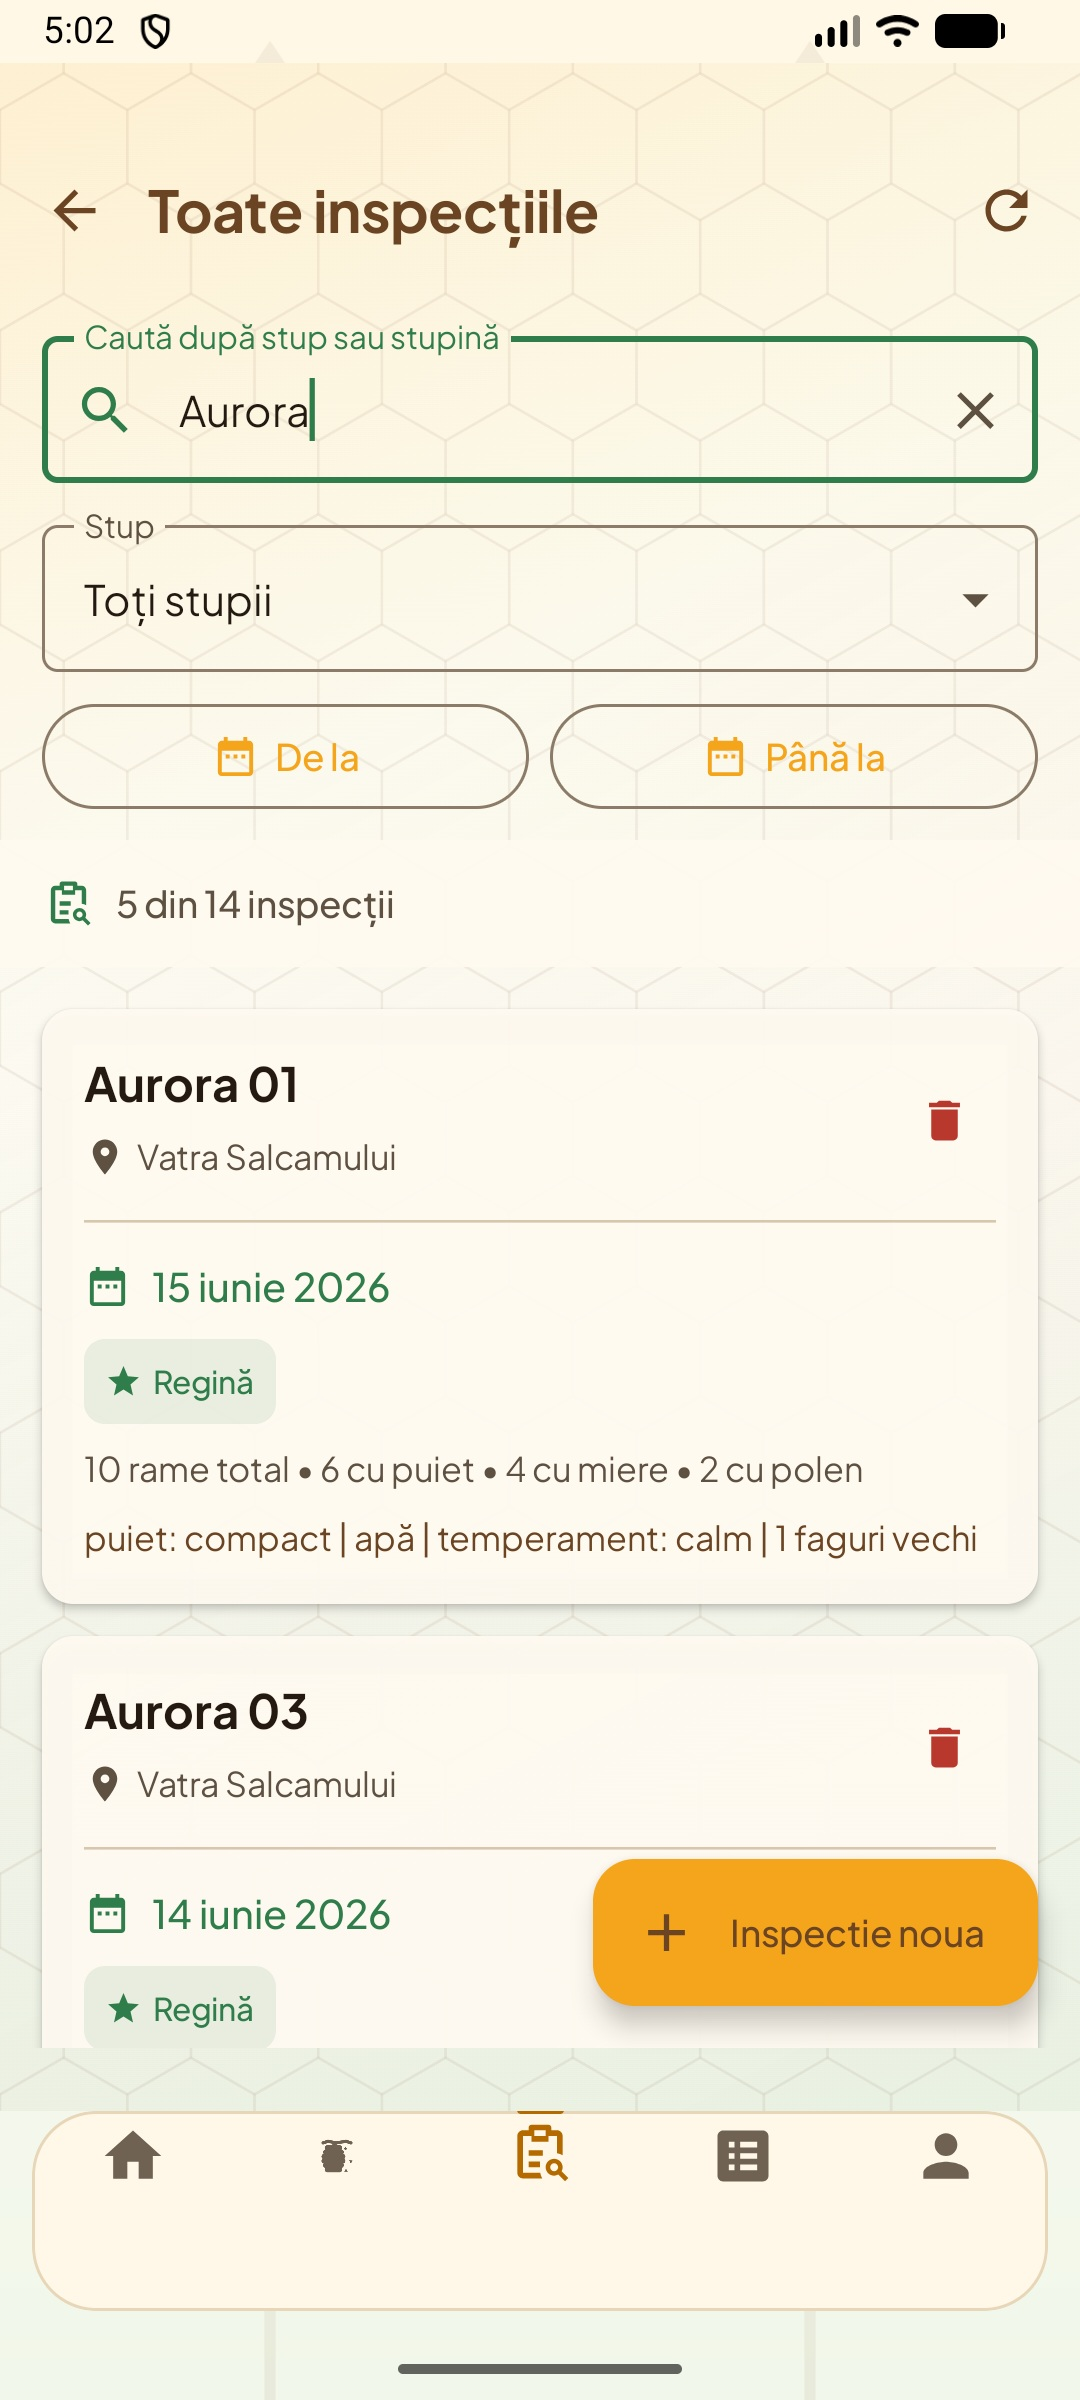
\includegraphics[width=0.40\textwidth]{./images/screenshots/inspection-list-updated.jpg}
	\caption{Jurnalul de inspecții actualizat: utilizatorul poate căuta după stup sau stupină, poate filtra după stup și perioadă și poate vedea rapid indicatorii principali ai fiecărei verificări.}
	\label{fig:inspection-list}
\end{figure}

Formularul a fost extins cu 13 câmpuri suplimentare care permit capturarea unui context mai complet al stării familiei. Utilizatorul poate marca botcile observate, botcile cu ouă (semnal direct de pregătire a roirii), aglomerarea sau barba la urdiniș, spațiul insuficient în stup, tiparele de puiet (compact, dispersat etc.), procentul mierii căpăcite, hrănirea efectuată în ziua inspecției, disponibilitatea apei, prezența umidității sau mucegaiului, albinele moarte la urdiniș, comportamentul neobișnuit al coloniei, temperamentul acesteia și numărul de faguri vechi care trebuie înlocuiți. Aceste date sunt salvate în aceeași entitate de inspecție, atât local, cât și pe server, și sunt folosite ulterior de advisorul contextual pentru generarea sfaturilor.


Formularul permite adăugarea de fotografii. Fotografiile pot fi realizate cu camera sau selectate din galerie, apoi sunt procesate de \texttt{PhotoManager}. În fluxul actual, fotografia este transformată în Base64 și trimisă ca Data URI. Dacă inspecția este salvată offline, fotografiile sunt memorate local și sincronizate după ce inspecția părinte primește id de server.

Utilizatorul poate rula analiza AI pentru o fotografie individuală, pentru fotografiile selectate sau pentru toate fotografiile atașate inspecției. Dacă backend-ul este disponibil, imaginea este trimisă la endpoint-ul \texttt{analyze-cells}. Rezultatul este afișat în dialogul de previzualizare al fotografiei, unde utilizatorul vede numărul de celule detectate, câte au coordonate, nivelul de încredere și raportul orientativ generat de \texttt{BroodAnalyzer}. Răspunsul poate fi:
\begin{itemize}
	\item \texttt{success}, dacă analiza a reușit;
	\item \texttt{low\_quality}, dacă fotografia este prea mică, neclară, prea întunecată, supraexpusă sau cu contrast insuficient;
	\item \texttt{not\_comb\_image}, dacă nu se detectează suficiente celule de fagure;
	\item \texttt{uncertain\_analysis}, dacă modelul are încredere scăzută în prea multe celule.
\end{itemize}

După succes, \texttt{BroodAnalyzer} transformă rezultatele în raport. Raportul poate evidenția semnale pozitive, precum prezența simultană a ouălor, larvelor și puietului căpăcit, sau semnale de atenție, precum lipsa larvelor ori rezerve scăzute. Aceste mesaje sunt orientative și trebuie interpretate împreună cu observația apicultorului. Rezultatul analizei DeepBee, așa cum este afișat în aplicație, este prezentat în figura~\ref{fig:ai-result}.

\begin{figure}[H]
	\centering
	\subfigure[Rezumatul analizei pe fotografie]{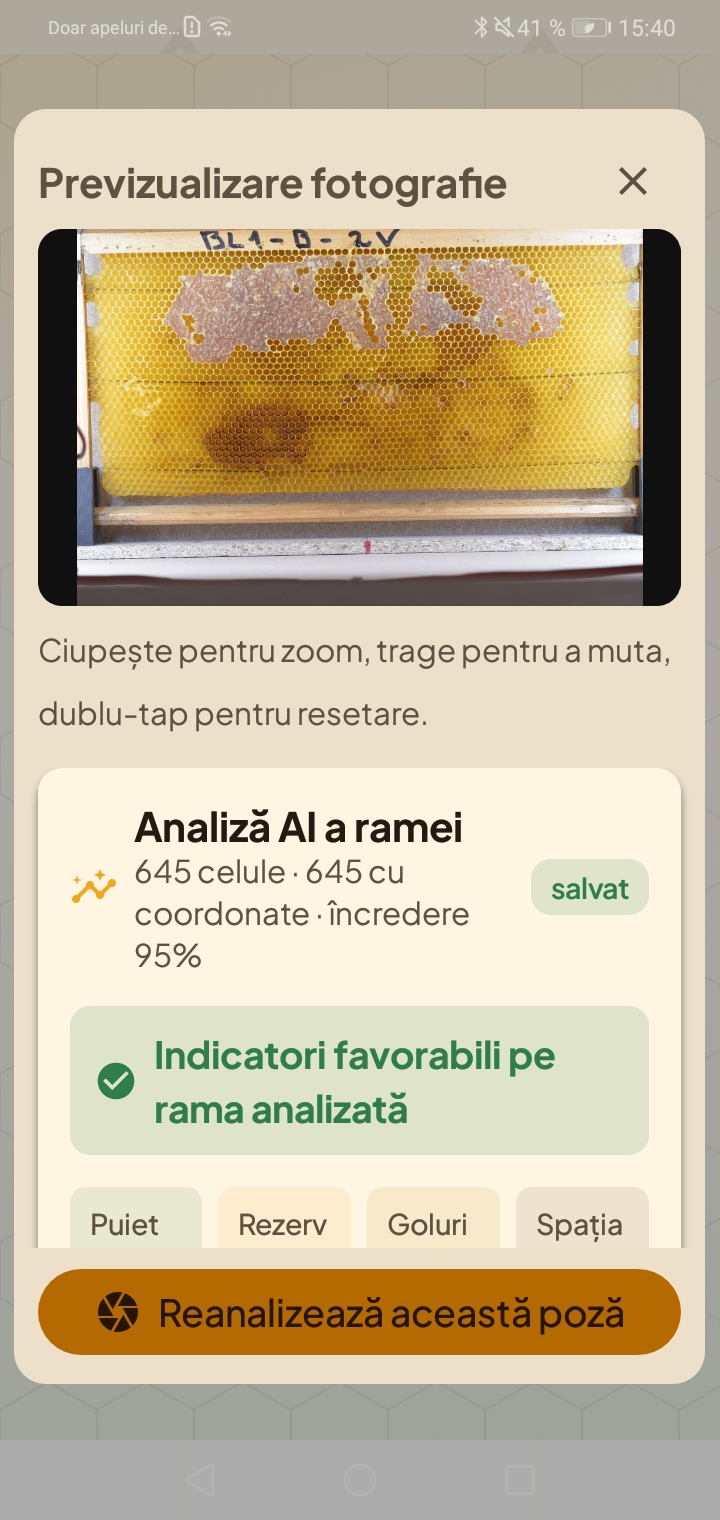
\includegraphics[width=0.40\textwidth]{./images/screenshots/ai-photo-preview-summary.jpg}}
	\hfill
	\subfigure[Detalii și pași recomandați]{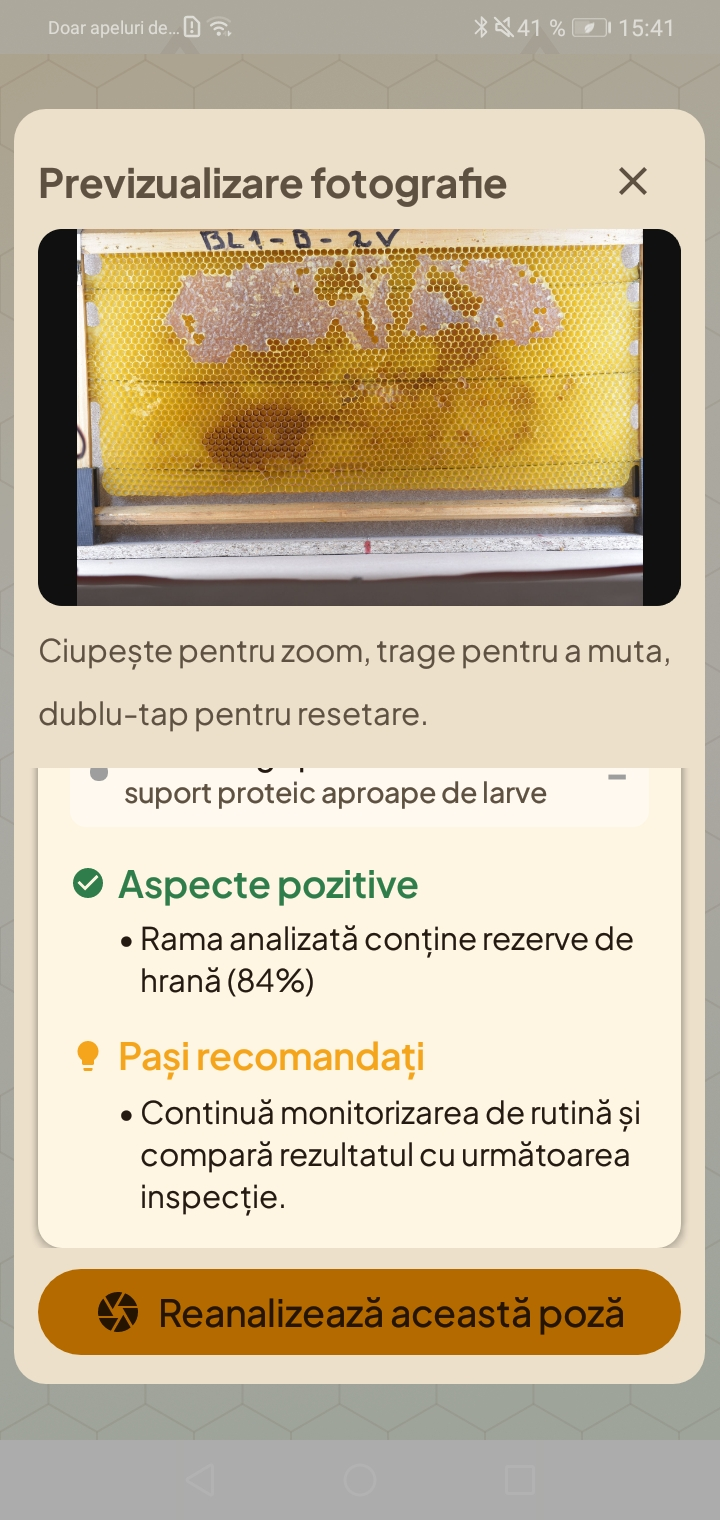
\includegraphics[width=0.40\textwidth]{./images/screenshots/ai-photo-preview-details.jpg}}
	\caption{Previzualizarea fotografiei de ramă după analiza AI: aplicația afișează numărul de celule detectate, existența coordonatelor, încrederea medie, verdictul orientativ, aspectele pozitive și pașii recomandați.}
	\label{fig:ai-result}
\end{figure}

\section{Vizualizarea statisticilor pe stup}

Pentru fiecare stup, aplicația poate afișa un raport DeepBee longitudinal. Ecranul \texttt{HiveStatsScreen} pornește de la analizele AI salvate și calculează puncte de sănătate pe luni. Utilizatorul vede numărul de celule analizate, indexul curent, puietul, rezervele și tendința față de analiza precedentă.

Ecranul include două tipuri de vizualizare:
\begin{itemize}
	\item evoluția lunară pentru anul curent, utilă pentru urmărirea sezonului;
	\item comparația inter-anuală pentru aceeași lună, utilă pentru observarea diferențelor de la un an la altul.
\end{itemize}

În plus, ultima analiză este detaliată prin distribuția celulelor și indicatori derivați. Această funcție transformă analiza AI dintr-un rezultat punctual într-un istoric utilizabil. Apicultorul nu vede doar \enquote{fotografia X a avut N celule}, ci poate observa dacă valorile se schimbă în timp. Raportul DeepBee longitudinal pe stup este ilustrat în figura~\ref{fig:hive-stats}.

\begin{figure}[H]
	\centering
	\subfigure[Indicatori longitudinali]{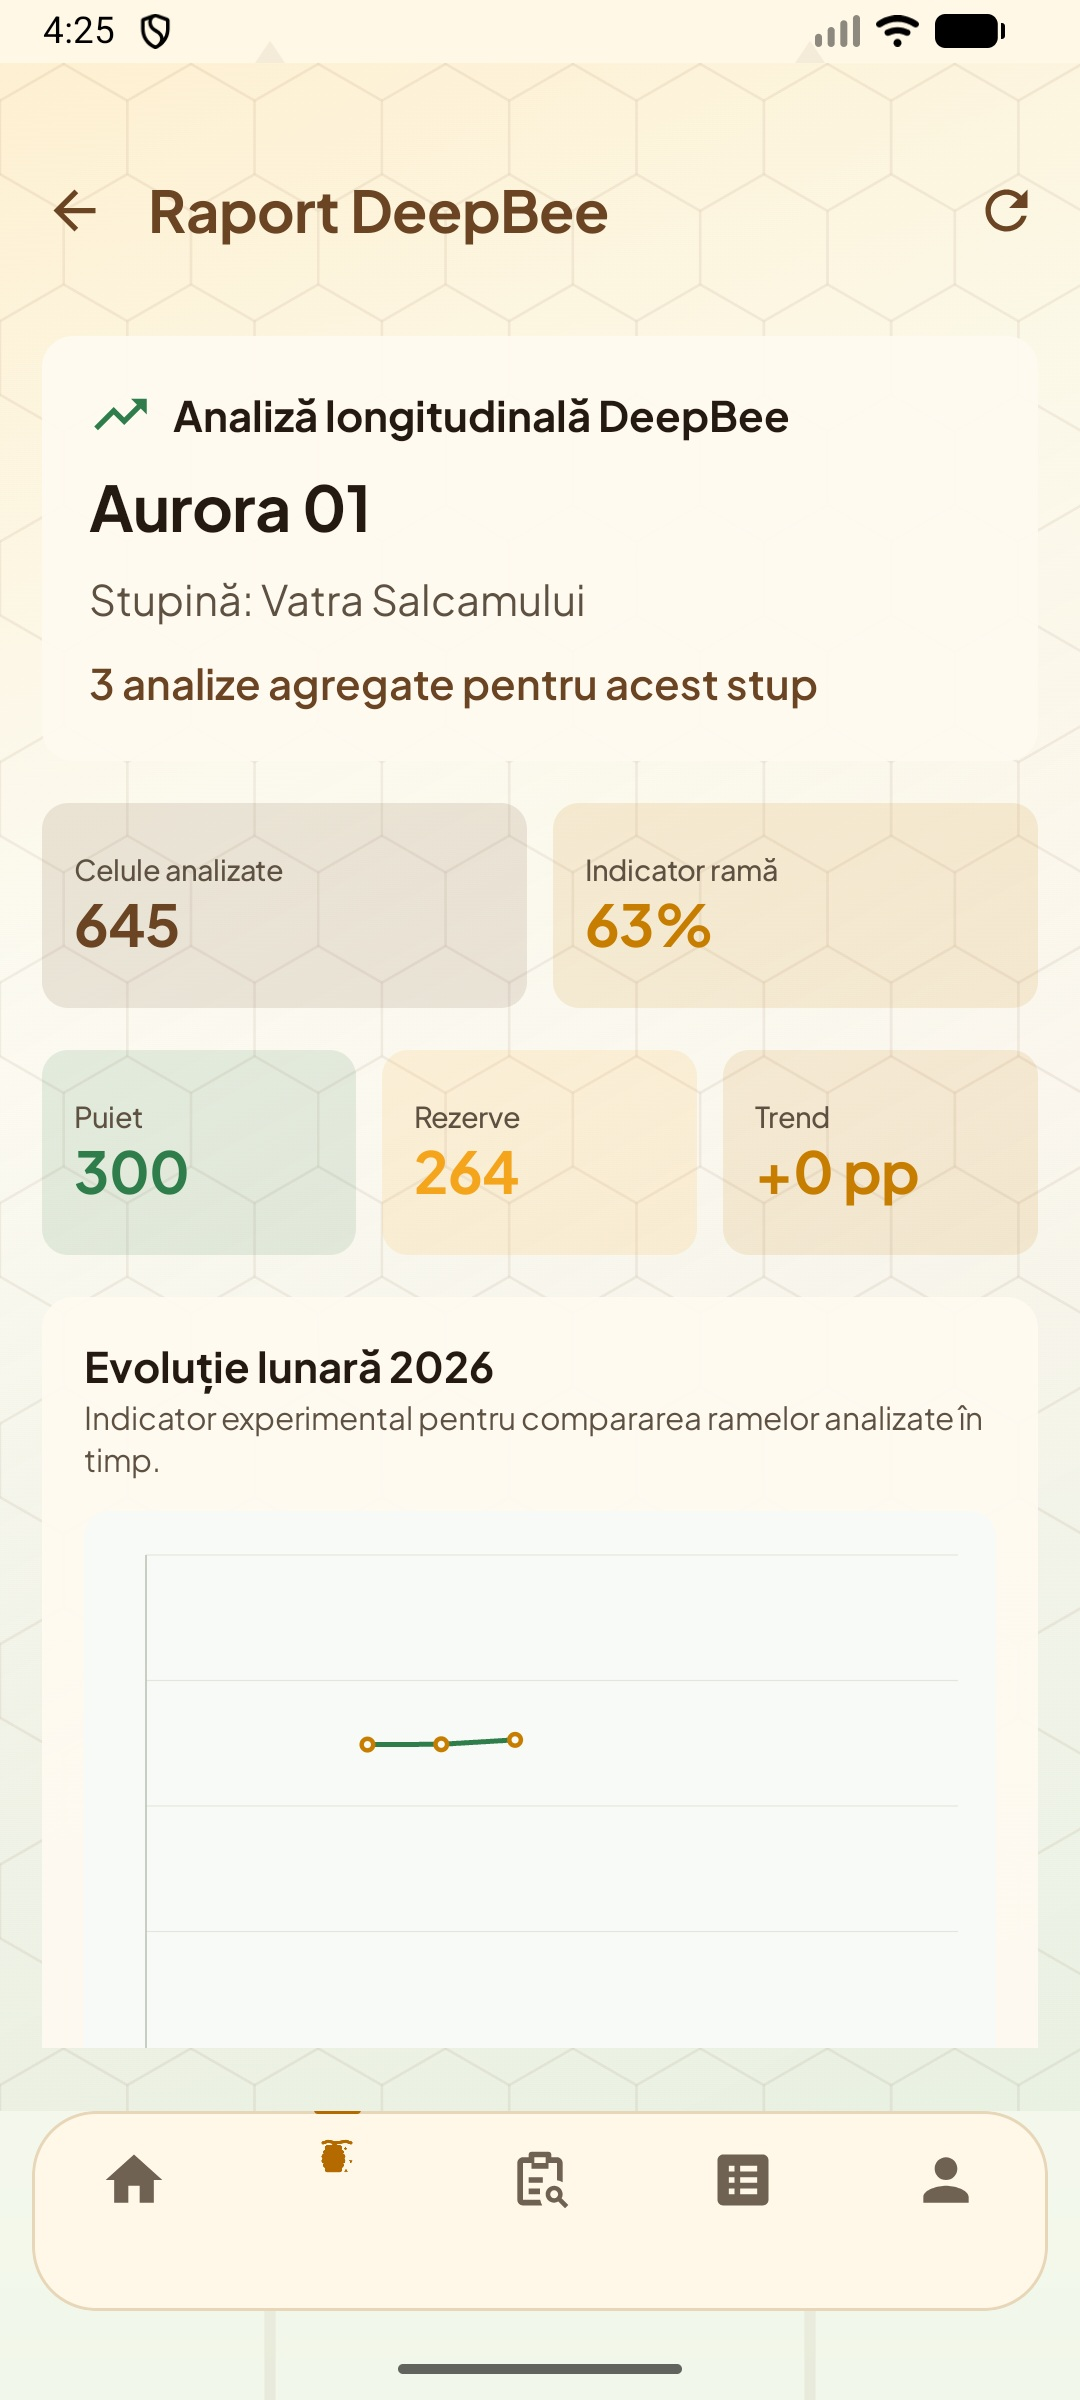
\includegraphics[width=0.40\textwidth]{./images/screenshots/hive-deepbee-stats-updated.jpg}}
	\hfill
	\subfigure[Distribuția ultimei analize]{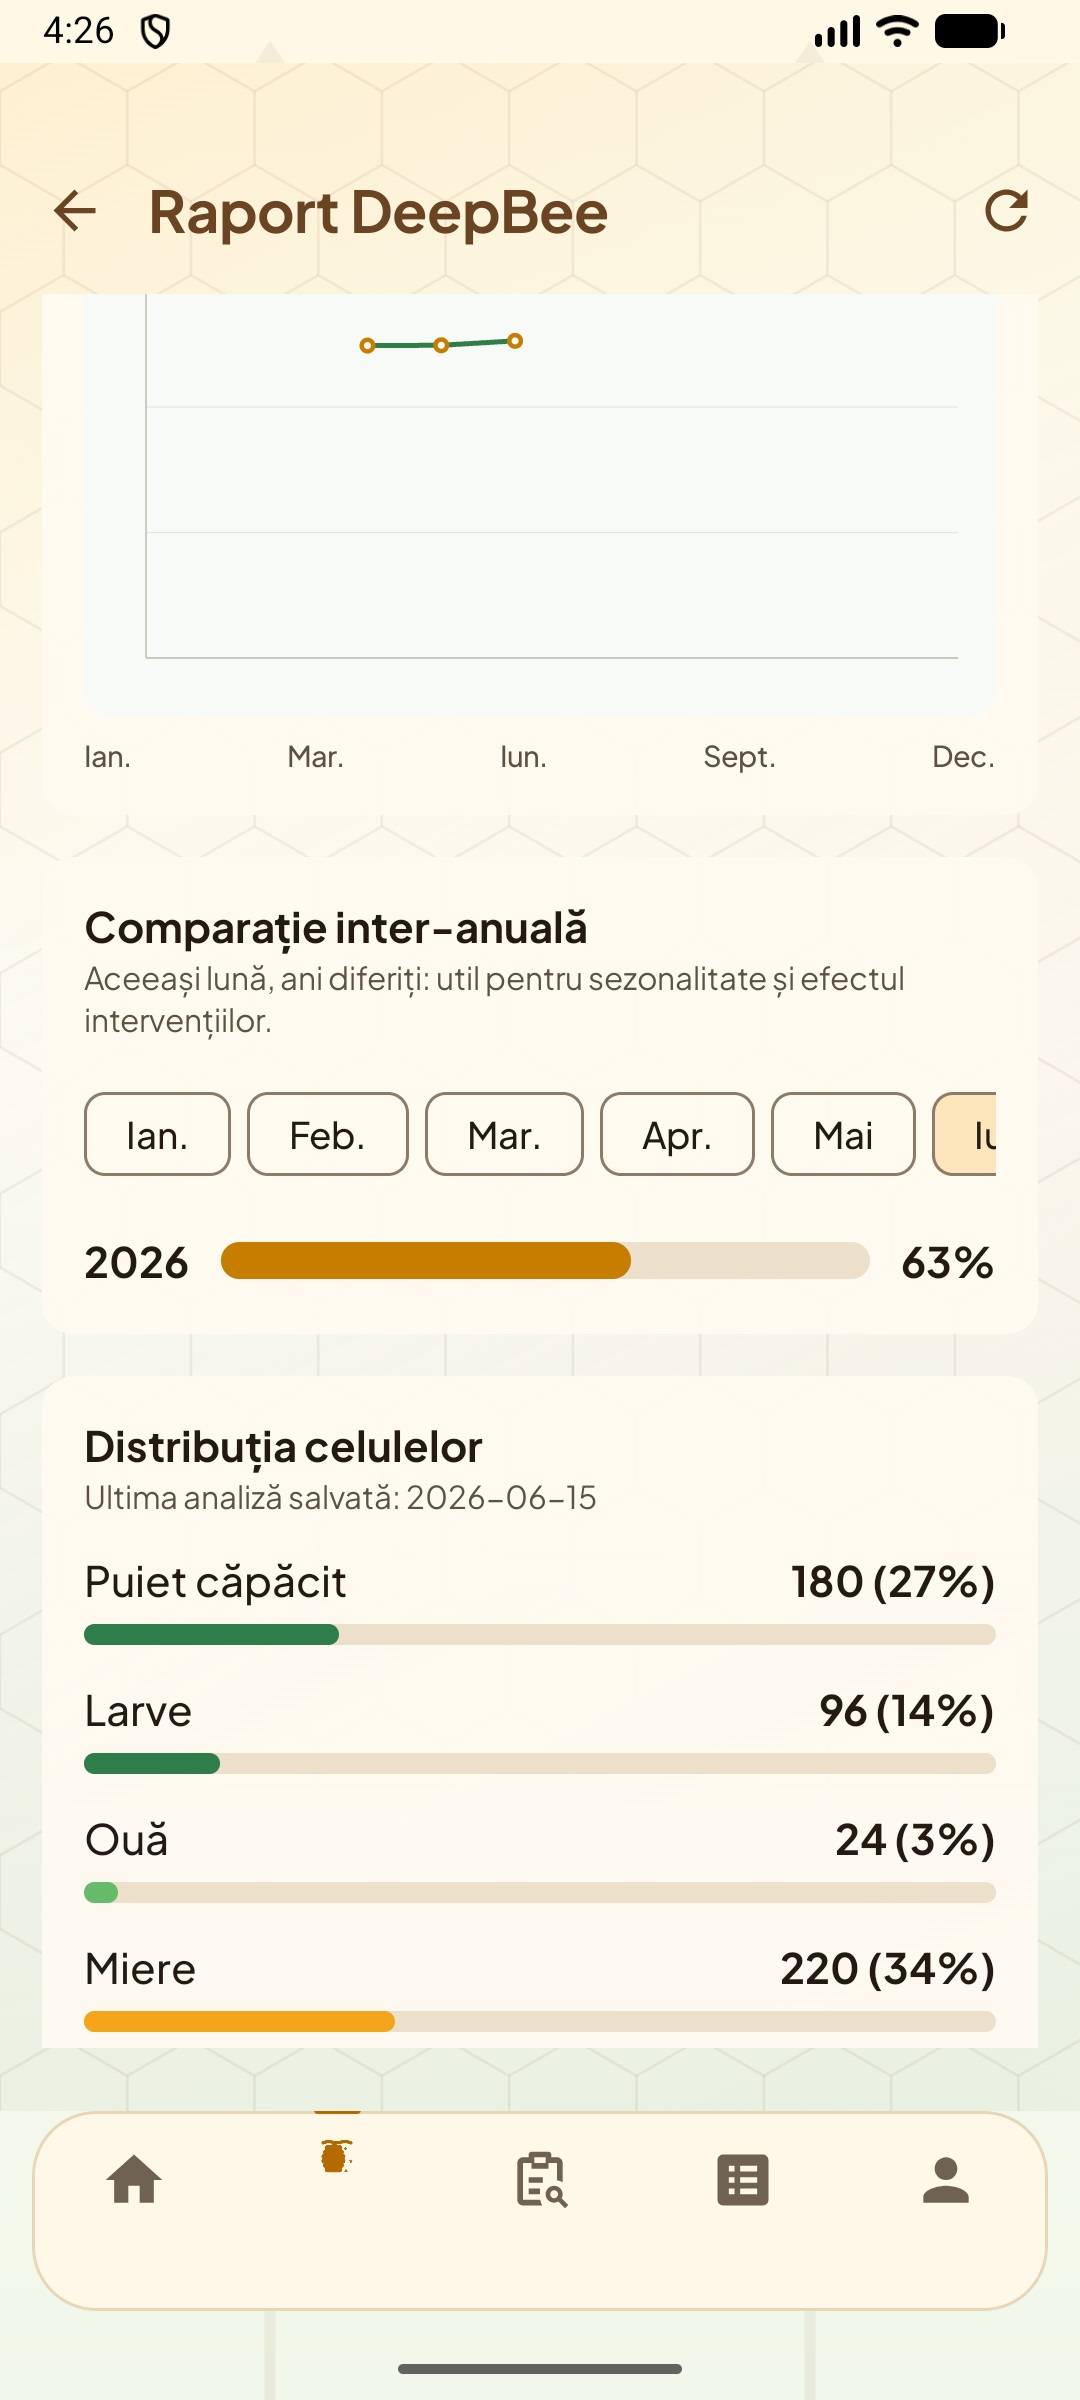
\includegraphics[width=0.40\textwidth]{./images/screenshots/hive-deepbee-distribution-updated.jpg}}
	\caption{Raportul DeepBee longitudinal pentru un stup: numărul de analize agregate, celulele analizate, indicatorul ramei, trendul lunar și distribuția pe categorii pentru ultima fotografie analizată.}
	\label{fig:hive-stats}
\end{figure}

\section{Dashboard cu analytics la nivel de stupină}

Ecranul principal al aplicației include un set de carduri cu indicatori calculați la nivel de stupină, actualizați la fiecare încărcare a ecranului. Aceste date sunt produse local de \texttt{DashboardAnalyticsCalculator} și nu necesită un apel suplimentar la server.

\begin{figure}[H]
	\centering
	\subfigure[Index de sănătate și plan recomandat]{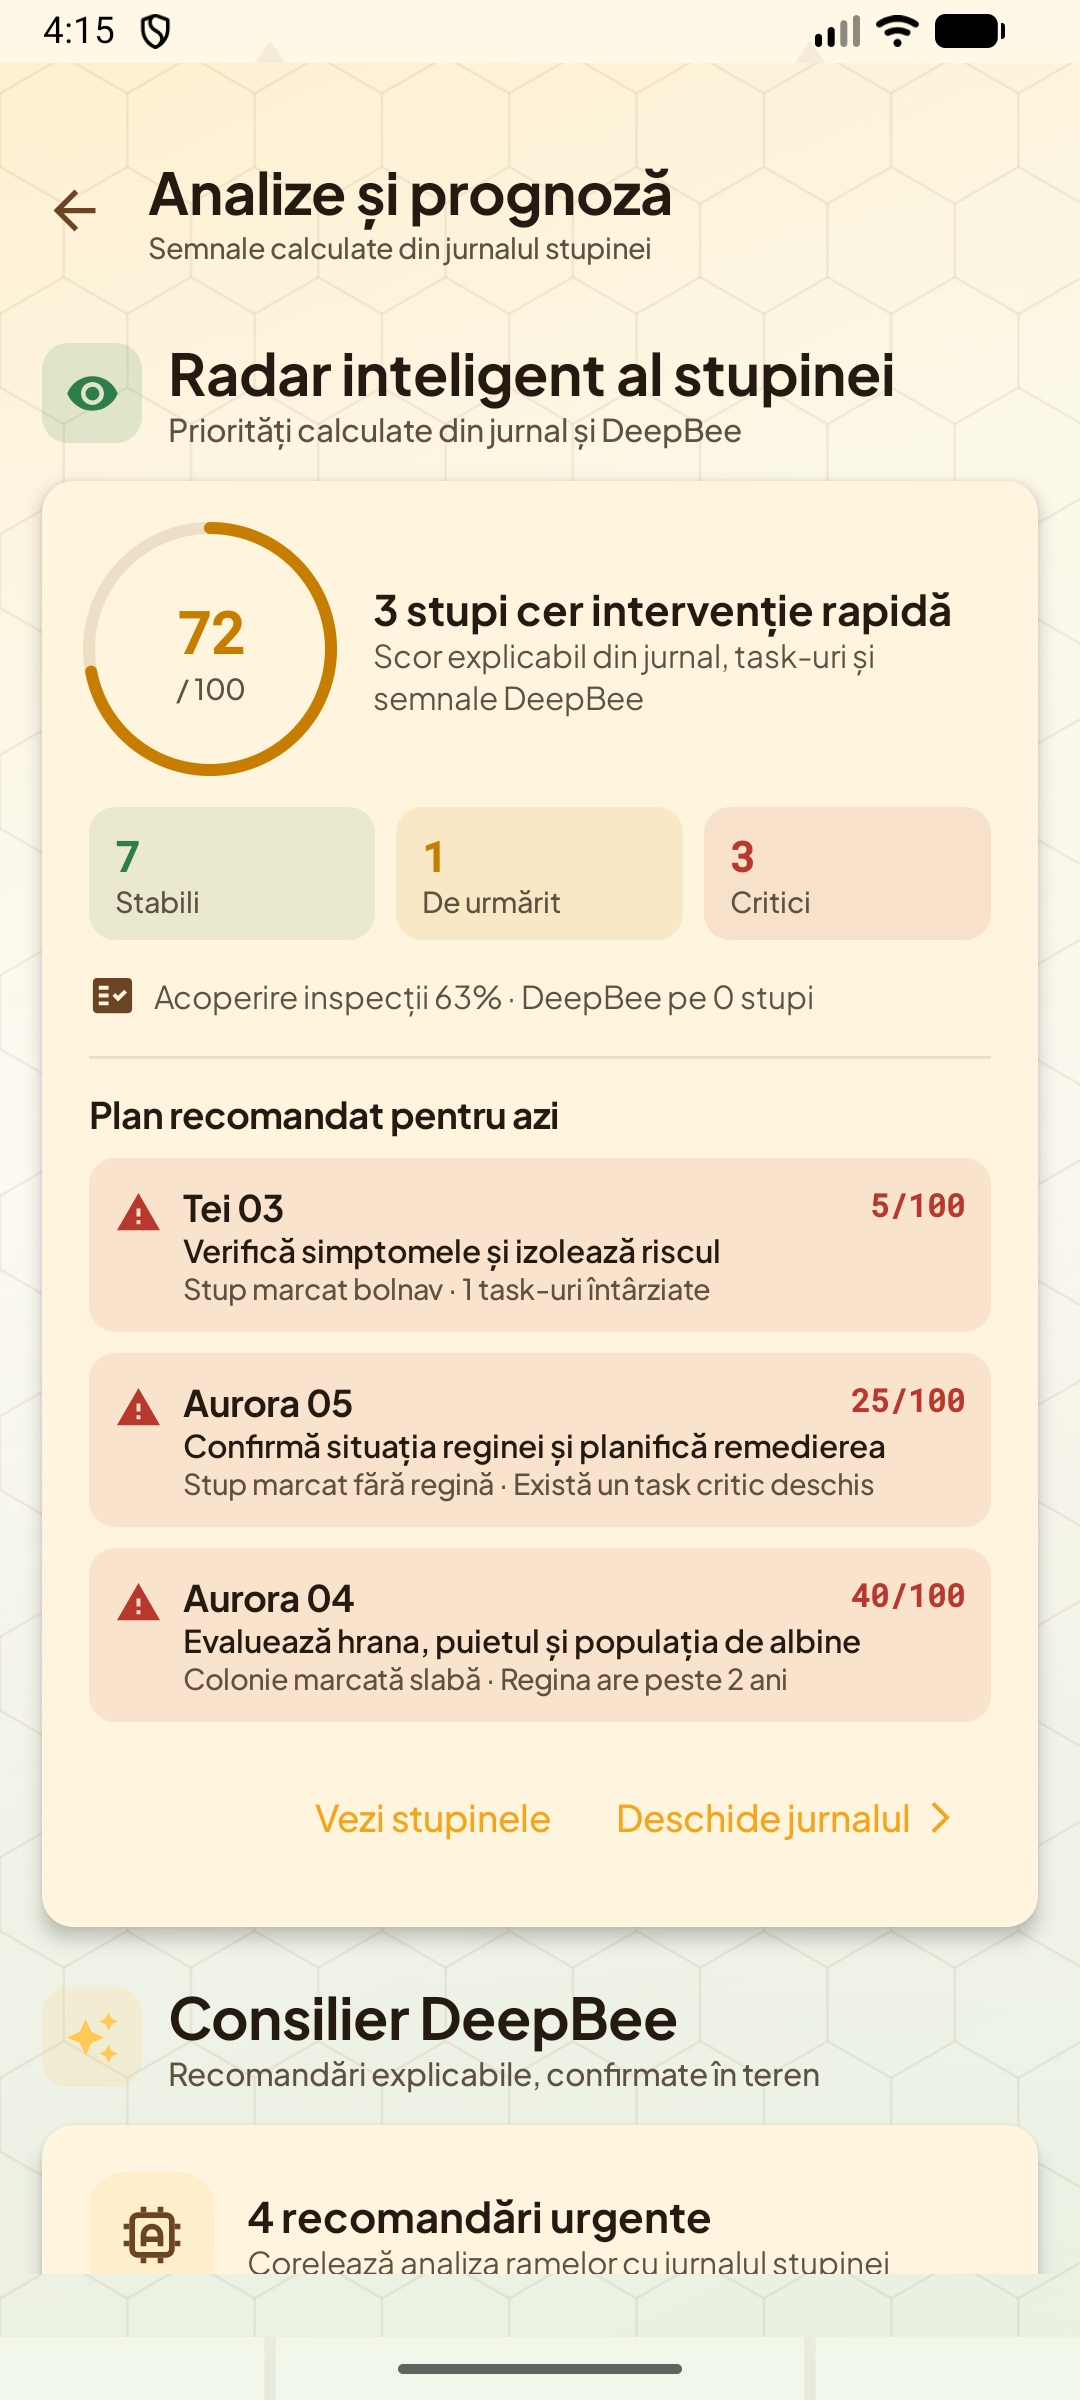
\includegraphics[width=0.40\textwidth]{./images/screenshots/dashboard-radar-updated.jpg}}
	\hfill
	\subfigure[Stupinele cu meteo și stare]{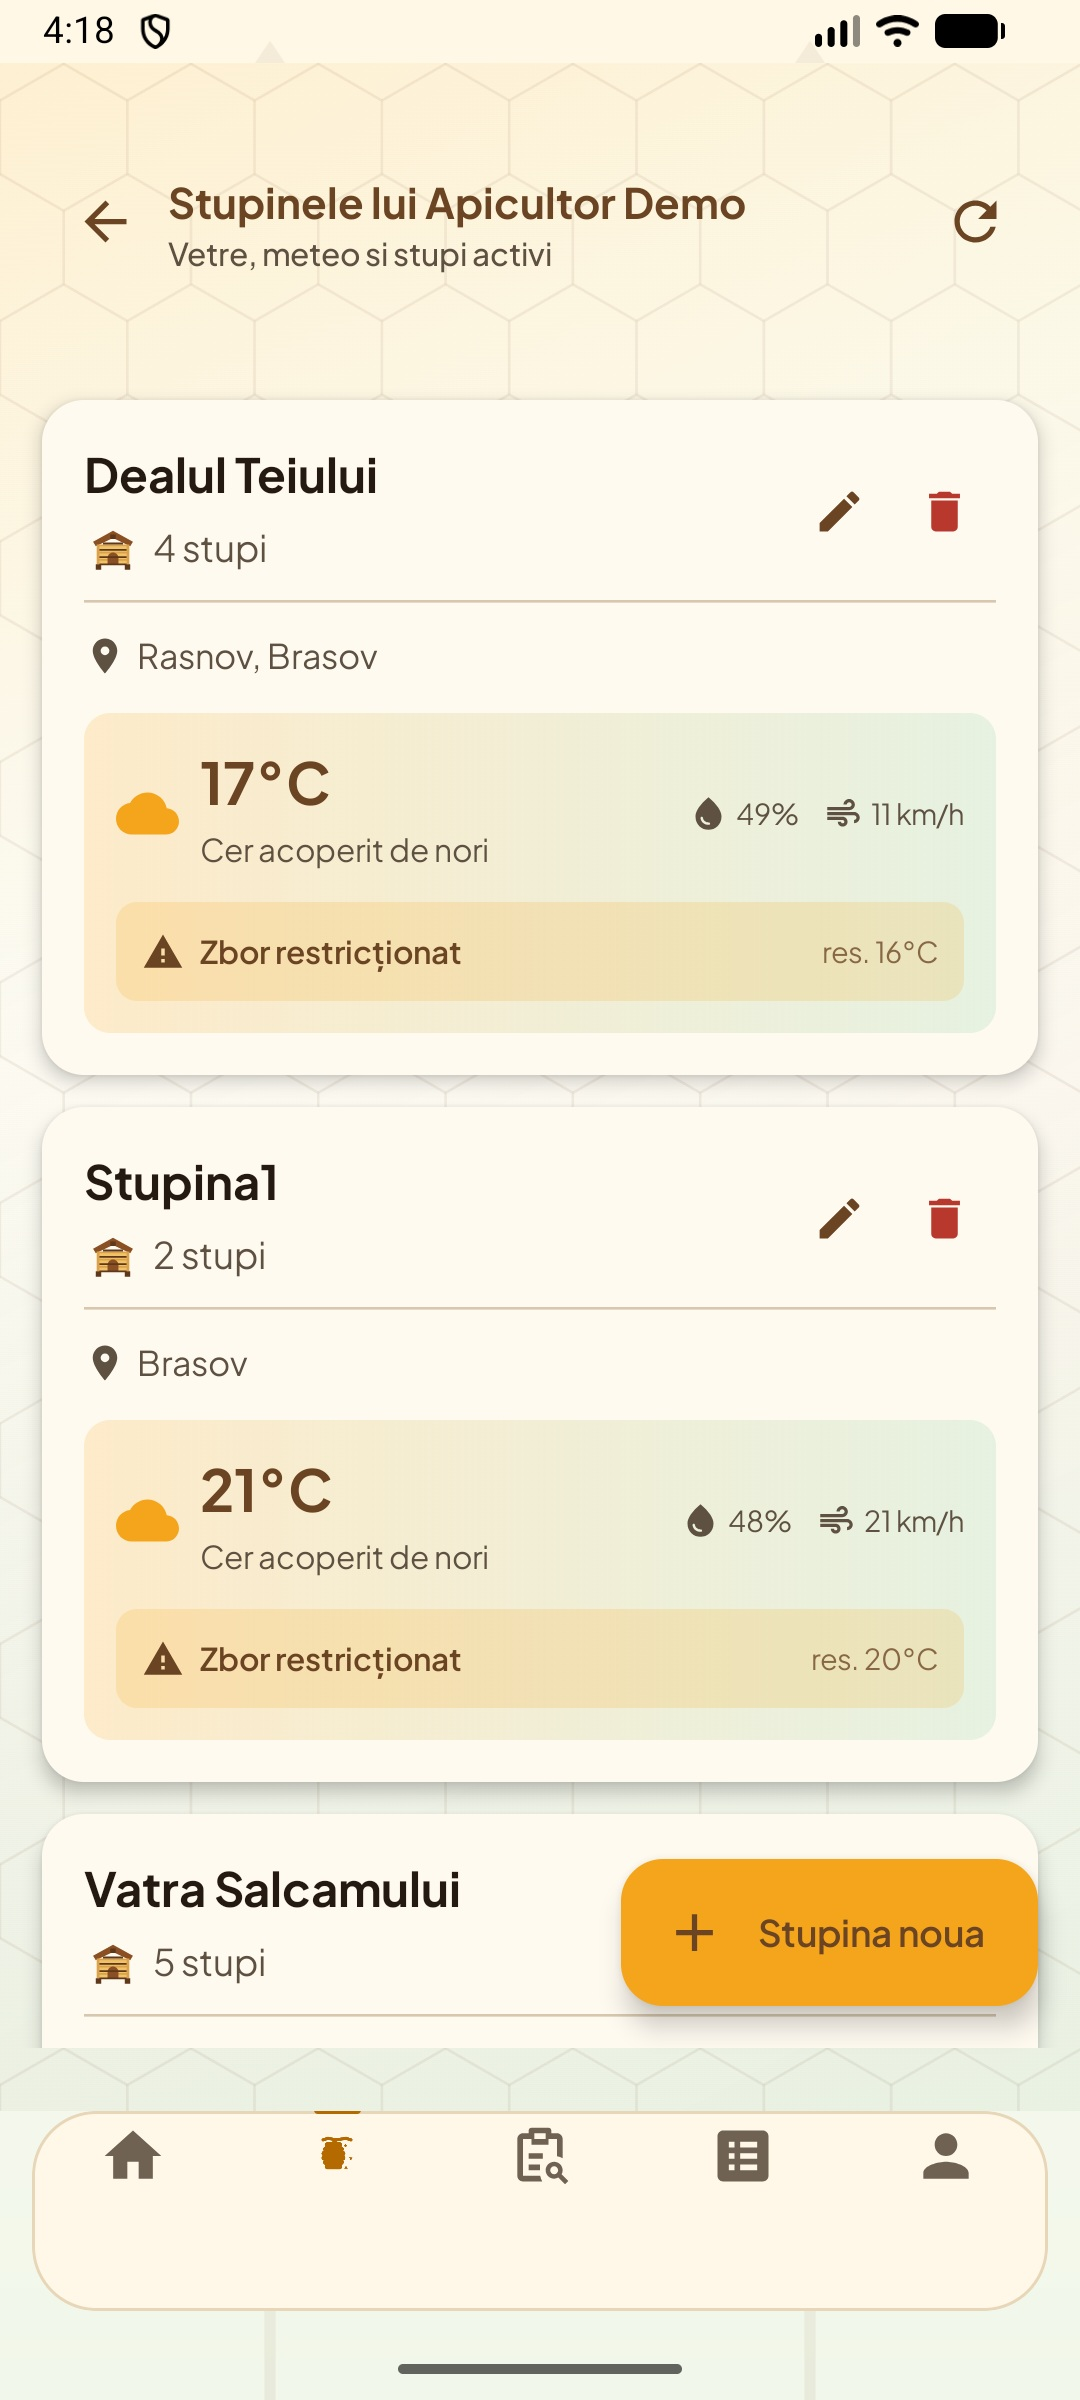
\includegraphics[width=0.40\textwidth]{./images/screenshots/14-apiaries-populated-updated.jpg}}
	\caption{Dashboard-ul cu analytics la nivel de stupină: indexul de sănătate cu planul recomandat și lista stupinelor cu date meteo contextuale.}
	\label{fig:dashboard}
\end{figure}


Un prim card afișează indexul de sănătate agregat al stupinei: scorul mediu, numărul de stupi \texttt{STABLE}, \texttt{WATCH} și \texttt{CRITICAL}, procentul stupilor cu inspecții recente și numărul celor cu cel puțin o analiză DeepBee. Sub aceste rezumate este afișată lista stupilor care necesită atenție, cu motivele penalizărilor și acțiunile sugerate.

Un al doilea card prezintă analiza de producție: producția de miere extrasă în anul curent, producția pe toată durata de viață a stupinei, prognoza pentru recolta iminentă (exprimată ca interval minim--mediu--maxim) și prognoza de sezon calculată prin adăugarea estimării ramelor cu miere la producția deja extrasă. Tendința de producție față de trimestrul anterior este exprimată procentual. Nivelul de încredere al prognozei este afișat explicit: \texttt{LOW} când datele sunt puține, \texttt{MEDIUM} sau \texttt{HIGH} pe măsură ce istoricul se acumulează.

Un al treilea card prezintă sfaturile \texttt{DeepBeeContextAdvisor}, grupate pe categorii (matcă, puiet, roire, nutriție, tratamente, producție, monitorizare, calitatea datelor) și ordonate după nivelul de urgență. Fiecare sfat include titlul, explicația, acțiunea propusă și dovezile extrase din datele aplicației. Utilizatorul poate citi sfatul și decide independent dacă îl aplică sau nu, fără ca aplicația să genereze alarme automate sau să prescrie acțiuni obligatorii. Cardurile de analytics ale dashboard-ului sunt prezentate în figura~\ref{fig:dashboard}.


\section{Tratamente, extracții și task-uri}

Tratamentele permit înregistrarea produsului administrat, substanței, dozei, datei și unei eventuale date de tratament următor. Tipurile de tratament includ, în modelul backend, Varroa, Nosema, fungal, viral, bacterial, preventive și other. Aceste informații ajută la păstrarea istoricului sanitar al stupului și sunt folosite de \texttt{DeepBeeContextAdvisor} pentru a verifica existența unui tratament Varroa înregistrat și termenele expirate.

Dacă un tratament are o dată de reaplicare, \texttt{TreatmentNotificationScheduler} programează automat o alarmă locală pentru ora 08:00 a zilei respective. Alarma supraviețuiește modului de economisire a energiei și, prin \texttt{BootCompleteReceiver}, și repornirii dispozitivului. Utilizatorul primește astfel o notificare în ziua planificată, fără a fi nevoie să verifice manual aplicația.

Extracțiile permit înregistrarea producției. Modelul include data extracției, tipul produsului, cantitatea, unitatea și notițe. Tipurile suportate includ miere, polen, propolis, lăptișor de matcă, ceară și altele. \texttt{DashboardAnalyticsCalculator} folosește înregistrările de extracții de tip \texttt{Honey} pentru calculul producției anuale și al prognozei de sezon.

Task-urile sunt folosite pentru planificarea lucrărilor. Ele pot fi asociate unei stupine sau unui stup și pot avea prioritate, status și termen limită. Pe Android, task-urile pot declanșa notificări locale prin \texttt{TaskNotificationScheduler}. De asemenea, \texttt{SyncManager} are operații speciale \texttt{COMPLETE} și \texttt{UNCOMPLETE}, pentru sincronizarea schimbării statusului unei sarcini.

\begin{figure}[H]
	\centering
	\subfigure[Task-uri prioritizate]{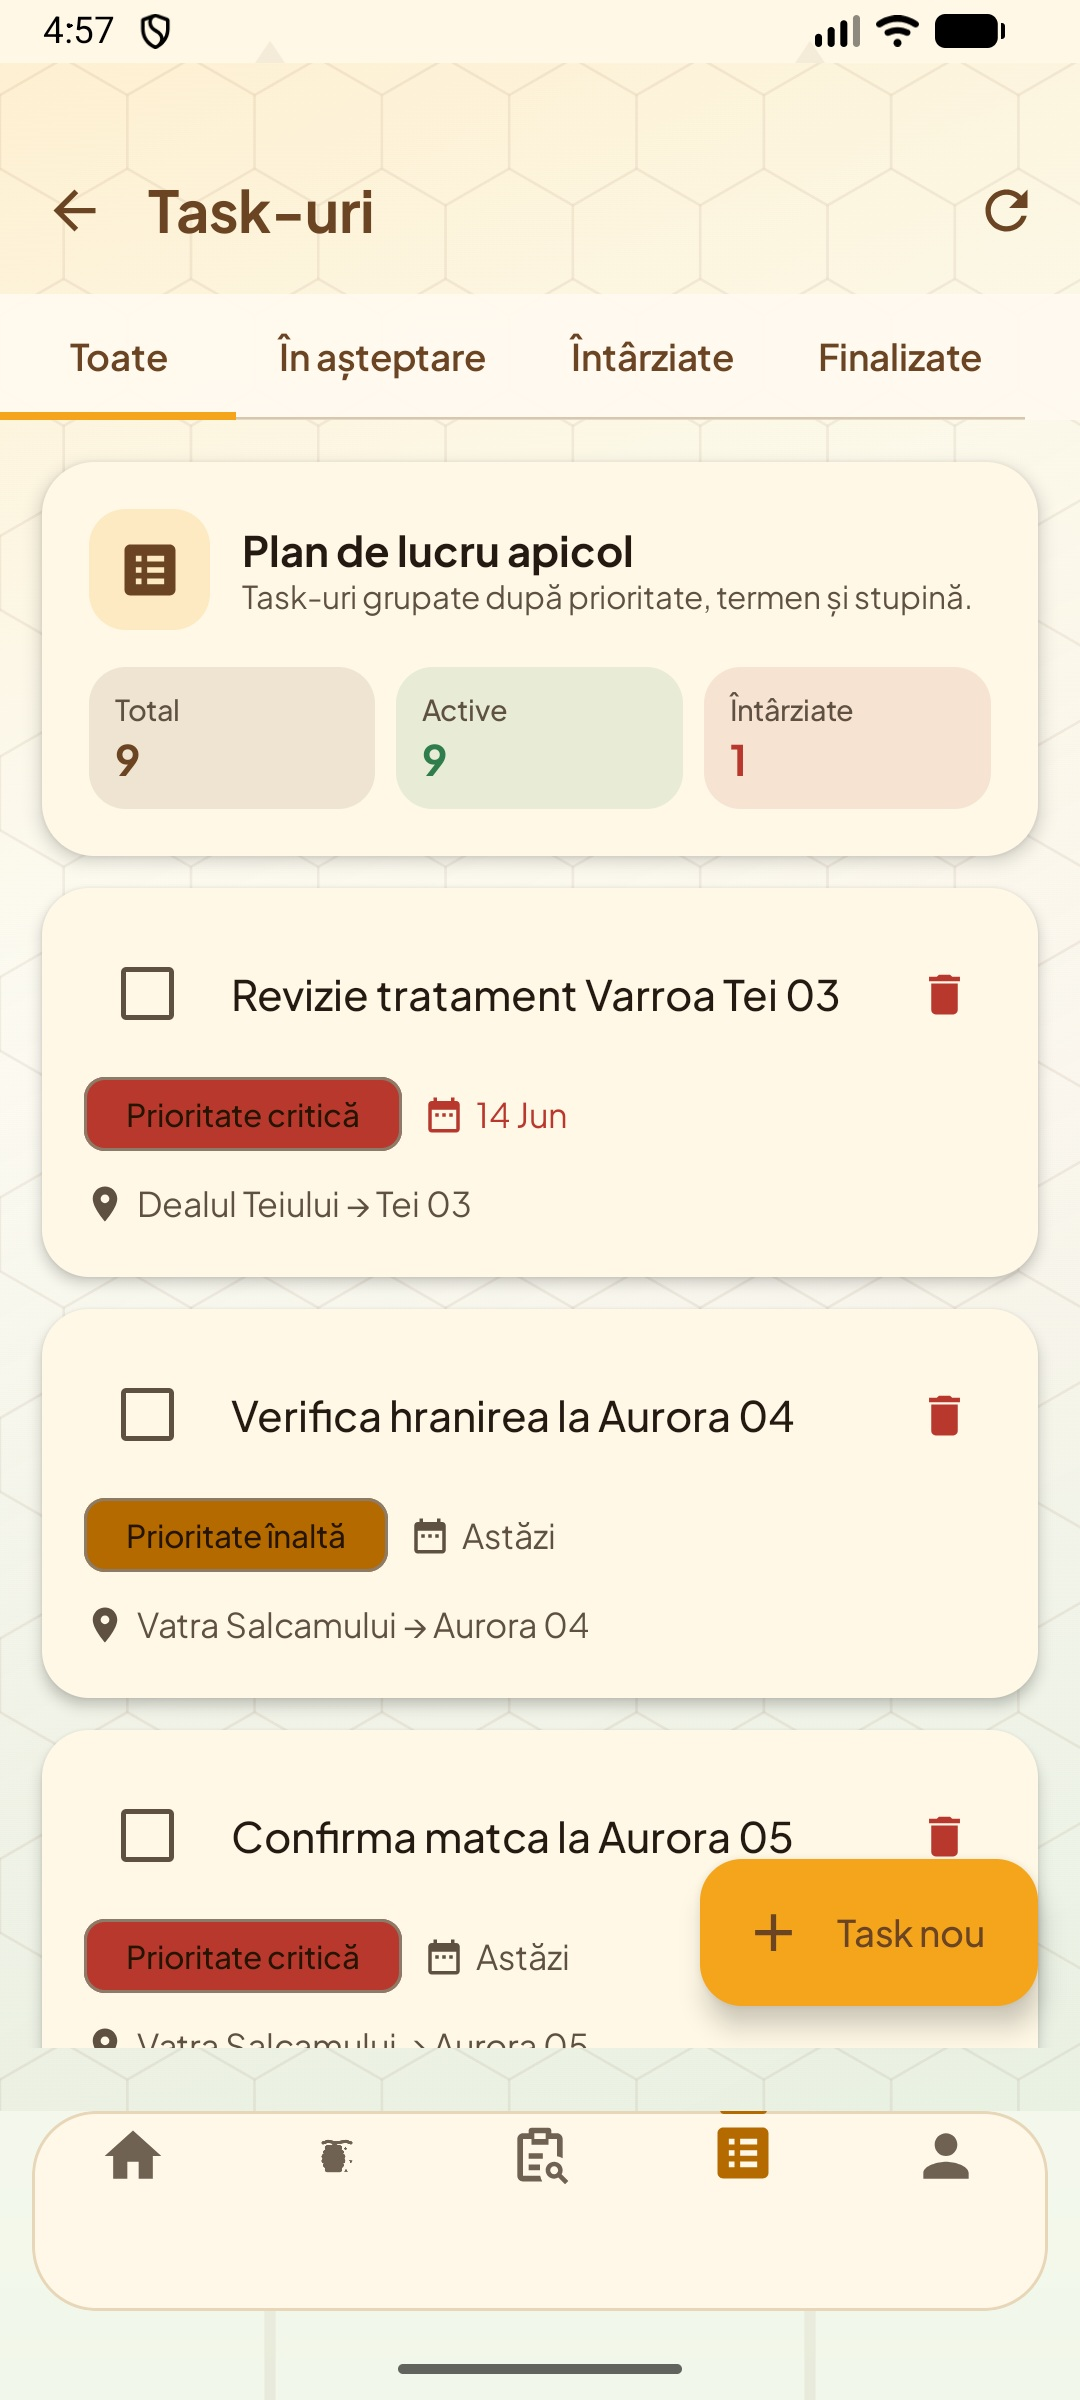
\includegraphics[width=0.40\textwidth]{./images/screenshots/task-list-updated.jpg}}
	\hfill
	\subfigure[Istoricul tratamentelor]{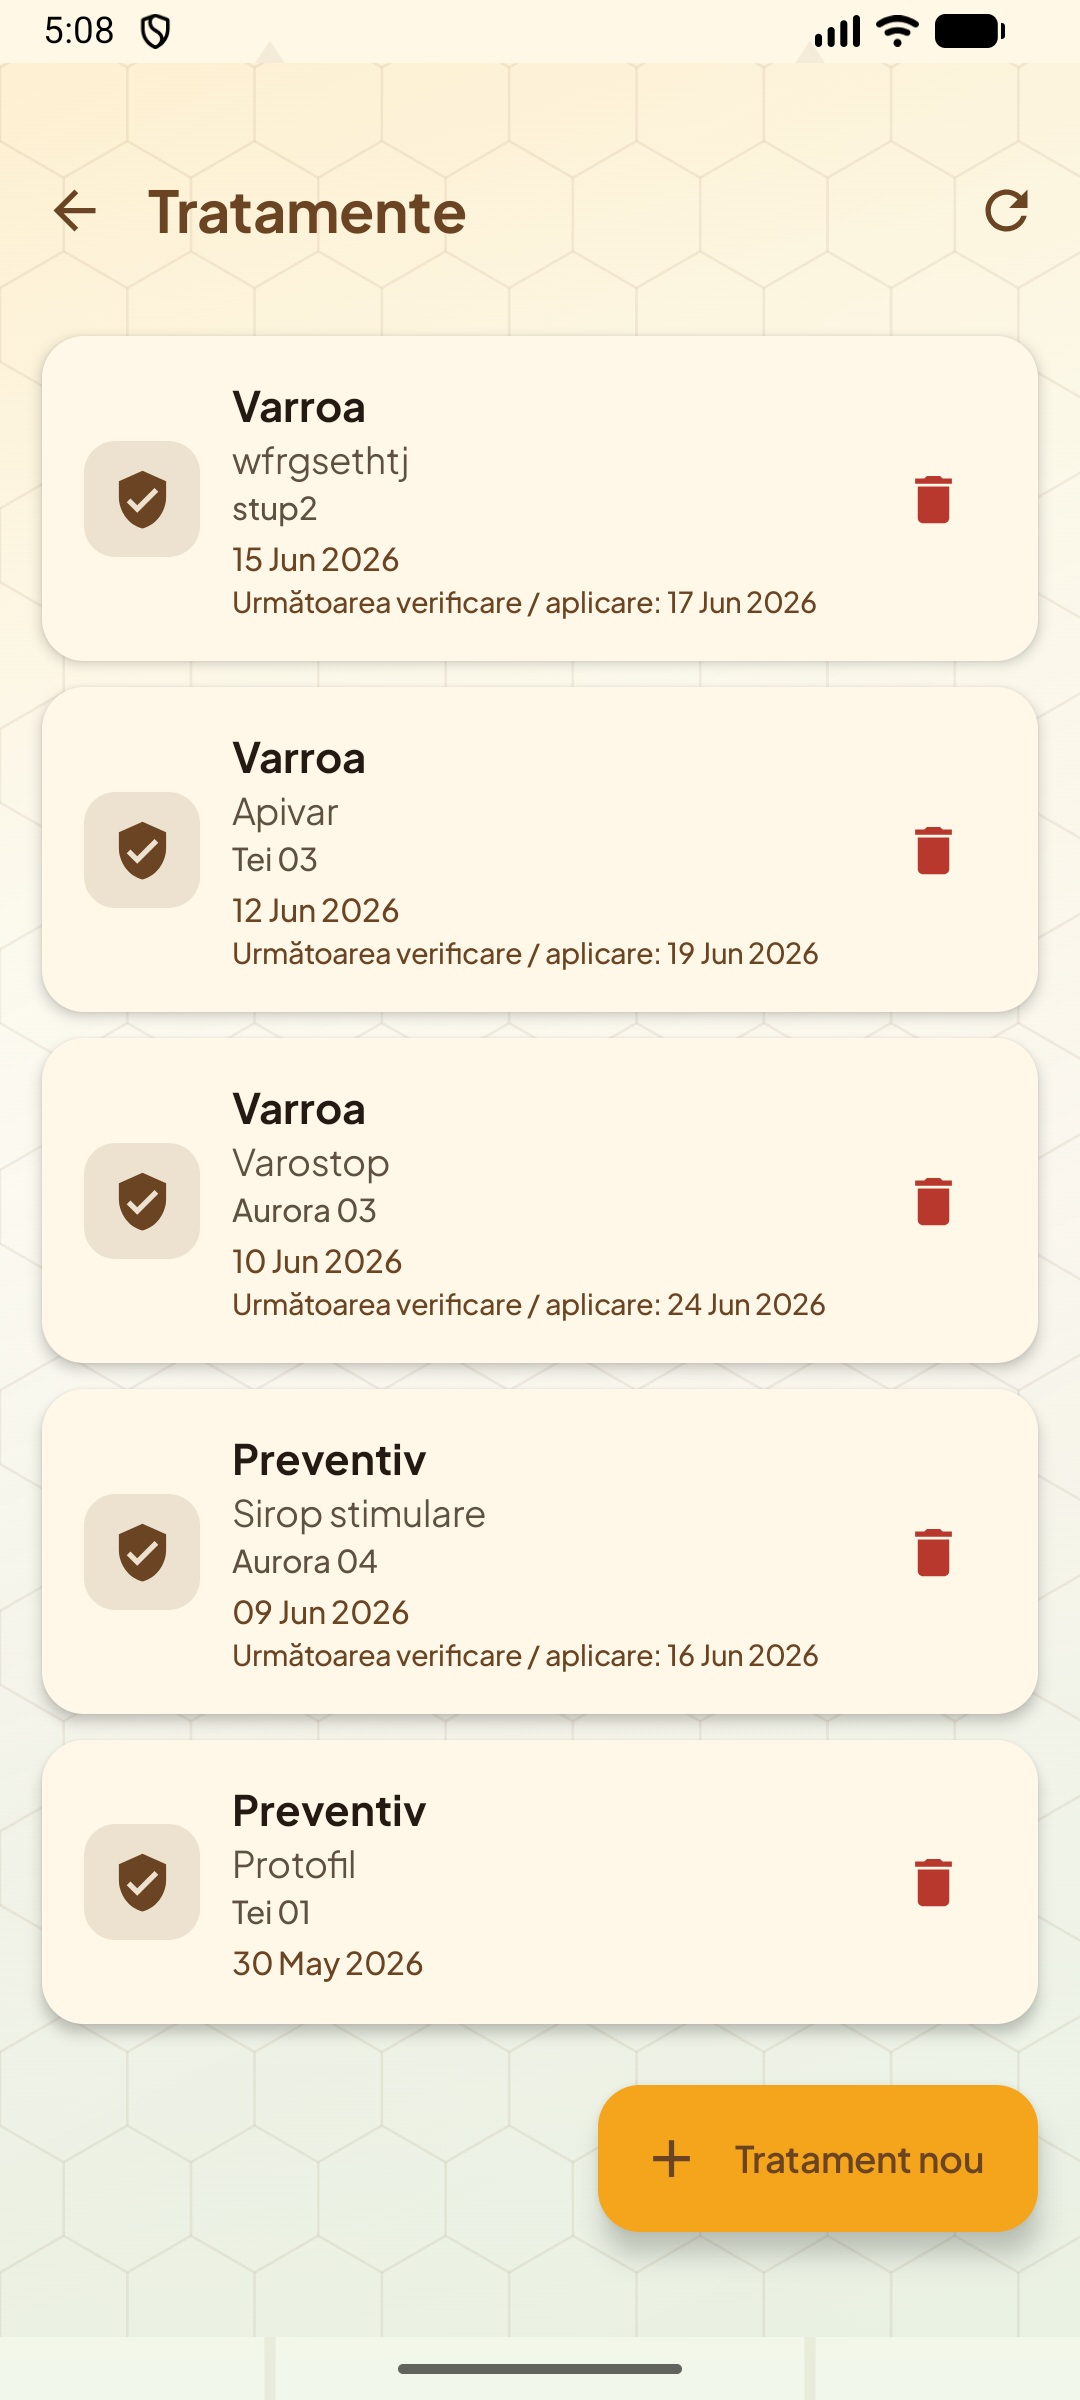
\includegraphics[width=0.40\textwidth]{./images/screenshots/treatment-list-updated.jpg}}
	\caption{Liste operaționale actualizate: task-urile sunt grupate după status și prioritate, iar tratamentele păstrează produsul, stupul, data aplicării și următoarea verificare.}
	\label{fig:worklists}
\end{figure}

\section{Funcționarea offline și sincronizarea}

Un scenariu important este lucrul complet offline. De exemplu, utilizatorul poate merge într-o stupină fără internet, poate crea o stupină nouă, adăuga doi stupi, completa inspecții și atașa fotografii. Toate aceste operații sunt salvate local. În acest timp, UI-ul nu este blocat, iar entitățile apar în liste.

Când dispozitivul revine online, \texttt{SyncScheduler} declanșează \texttt{SyncWorker}. Worker-ul apelează \texttt{SyncManager}, care procesează coada. Testele de integrare arată că ordinea este respectată: stupina este trimisă înaintea stupului, iar stupul înaintea inspecției sau fotografiei. Această ordine garantează că backend-ul primește id-uri valide.

Starea curentă a sincronizării poate fi consultată direct din ecranul de profil. \texttt{UserProfileScreen} afișează numărul de operații pendinte și momentul ultimei sincronizări confirmate cu serverul. Această informație ajută utilizatorul să știe dacă datele introduse în teren au ajuns pe server sau sunt încă în așteptare.

În cazul unei erori temporare, operația rămâne în coadă. În cazul unei erori repetate de server, entitatea este marcată \texttt{SYNC\_FAILED}. Într-o versiune viitoare, UI-ul ar putea afișa explicit o listă de operații eșuate, astfel încât utilizatorul să poată decide manual ce se întâmplă cu datele.

\section{Validare prin teste Android}

Partea Android include o infrastructură de teste orientată către sincronizarea offline-online. \texttt{SyncTestHarness} construiește o bază Room în memorie, un client Retrofit real, un MockWebServer și repository-uri reale. Astfel, testele verifică fluxul complet de la apelul repository-ului până la request-ul HTTP trimis către serverul mock.

Clasa \texttt{OfflineToOnlineSyncTest} acoperă scenarii fericite: creare de stupină offline și sincronizare, actualizare, ștergere, creare de stupină și stup în ordine de dependență, task-uri create peste părinți nesincronizați, tratamente și extracții. Clasa \texttt{SyncEdgeCasesTest} acoperă situații de eroare: retry-uri repetate, \texttt{IOException}, payload malformat, ștergeri 404, idempotency și părinți eșuați.

Pe lângă testele de integrare, există teste unitare pentru repository-uri individuale, pentru meteo, pentru \texttt{BroodAnalyzer}, pentru maparea statusurilor de analiză AI, pentru \texttt{ApiaryIntelligenceCalculator}, pentru \texttt{DashboardAnalyticsCalculator} și pentru \texttt{DeepBeeContextAdvisor}. Aceste teste verifică separat logica fiecărui calculator, inclusiv cazuri limită: stupi fără inspecții, snapshot-uri AI expirate, extracții cu unități nenormalizate, priorități de sfaturi și calendarul sezonier. Există și teste unitare pentru ViewModel-uri (\texttt{CreateApiaryViewModelTest}, \texttt{HiveFormViewModelTest}, \texttt{TaskFormViewModelTest}), care verifică comportamentul stărilor UI la acțiunile utilizatorului.

\section{Validare prin teste backend}

Backend-ul are un proiect separat de teste, \texttt{ApiaryServer.Tests}, care acoperă în prezent șapte seturi de scenarii.

Testele pentru \texttt{AuthController} verifică scenariile de înregistrare, login, confirmare email și resetare parolă, inclusiv cazuri de date invalide, email duplicat și token expirat. \texttt{AuthServiceTests} verifică logica serviciului de autentificare, inclusiv generarea și validarea token-urilor JWT și a refresh token-urilor.

Testele pentru \texttt{ApiaryService} verifică operații precum listare, creare, actualizare și ștergere, inclusiv cazul în care o stupină aparține altui utilizator. Testele pentru \texttt{HiveService} și \texttt{InspectionService} urmează același pattern: fiecare operație este testată atât pe calea fericită, cât și pentru cazurile de ownership incorect. \texttt{HiveTreatmentServiceTests} și \texttt{HiveExtractionServiceTests} verifică operațiile CRUD pe tratamente și extracții, inclusiv validarea tipurilor și a proprietarului resurselor. \texttt{TaskServiceTests} acoperă crearea, actualizarea, completarea și ștergerea task-urilor.

Testele pentru \texttt{AiAnalysisService} verifică modul în care serviciul C\# păstrează statusurile primite de la AIService. De exemplu, dacă serviciul AI întoarce \texttt{low\_quality} sau \texttt{not\_comb\_image}, backend-ul nu le transformă forțat în succes. De asemenea, dacă serviciul AI întoarce o eroare HTTP, \texttt{AiAnalysisService} aruncă o excepție care poate fi tratată de controller.

\texttt{AppDbContextModelTests} verifică că configurările de precizie zecimală din \texttt{AppDbContext} sunt aplicate corect la schema generată, astfel încât câmpurile cu mai mult de două zecimale (\texttt{BroodDensity}, \texttt{LarvaeToCappedRatio}, \texttt{StoresRatio}) să nu fie trunchiată la (18, 2) în mod implicit.

\section{Rezultate ale testării}

\begin{table}[H]
	\centering
	\begin{tabular}{l c p{4.7cm}}
		\hline
		\textbf{Suită} & \textbf{Nr. teste} & \textbf{Acoperire} \\
		\hline
		\texttt{ApiaryServer.Tests} (backend) & 101 & servicii, controllere, JWT, model BD \\
		Android (JVM / Robolectric) & 234 & sincronizare offline, repository-uri, calculatoare, ViewModel \\
		Android instrumentat & 1 & UI pe dispozitiv \\
		\hline
	\end{tabular}
	\caption{Sinteza suitelor de teste automate. Suita backend a fost executată integral (101 trecute, 0 eșuate).}
	\label{tab:teste-automate}
\end{table}

Suitele de teste automate au fost rulate înainte de predare. Proiectul de teste al backend-ului, \texttt{ApiaryServer.Tests}, a fost executat cu \texttt{dotnet test}: toate cele 101 de teste au trecut, fără niciun eșec. Suita Android, rulată cu \texttt{gradlew testDebugUnitTest}, cuprinde 234 de teste unitare și de integrare executate pe JVM (prin Robolectric și MockWebServer), plus un test instrumentat care necesită un dispozitiv sau emulator. Tabelul \ref{tab:teste-automate} sintetizează aceste suite.

Cele mai multe verificări pe Android se concentrează pe stratul de date și pe sincronizare, acolo unde o eroare ar însemna pierderea sau duplicarea datelor introduse în teren: scenariile offline-online, rezolvarea identificatorilor părinte-copil, politica de reîncercare și marcarea operațiilor eșuate. Restul suitei acoperă calculatoarele de indicatori, interceptorii de rețea și ViewModel-urile formularelor. Deoarece testele rulează pe JVM, prin Robolectric și MockWebServer, suita completă poate fi executată rapid, fără emulator, ceea ce a permis rularea ei frecventă pe parcursul dezvoltării, nu doar înainte de predare.

Pe partea de backend, ponderea mare a testelor de servicii reflectă decizia de a concentra logica de business în acest strat. Verificările de ownership apar pentru fiecare entitate, deoarece izolarea datelor între utilizatori este o cerință de securitate, nu o convenție opțională. Testele dedicate \texttt{AiAnalysisService} au un rol aparte: ele garantează că statusurile de calitate întoarse de serviciul AI ajung nealterate la client, adică exact comportamentul responsabil discutat în capitolul \ref{chap:suport-teoretic}.

\begin{table}[H]
	\centering
	\begin{tabular}{l l}
		\hline
		\textbf{Scenariu verificat manual} & \textbf{Rezultat} \\
		\hline
		Autentificare și înregistrare cont & Funcțional \\
		Dashboard cu indicatori (index de sănătate, plan recomandat) & Funcțional \\
		Listă de stupine cu date meteo contextuale & Funcțional \\
		Listă de stupi cu statusuri (activ, slab, fără regină) & Funcțional \\
		Jurnal de inspecții filtrat pe stup sau stupină & Funcțional \\
		Task-uri, tratamente și extracții populate în contul demo & Funcțional \\
		Fișa stupului și raportul longitudinal DeepBee & Funcțional \\
		Generarea codului QR pentru un stup & Funcțional \\
		Editarea profilului și sincronizarea cu serverul & Funcțional \\
		\hline
	\end{tabular}
	\caption{Scenarii verificate manual în aplicația Android, pe contul demo.}
	\label{tab:teste-manuale}
\end{table}

Tabelul \ref{tab:teste-manuale} prezintă scenariile verificate, ilustrate și de capturile din acest capitol. Verificarea manuală a fost realizată pe un telefon fizic, cu aplicația conectată la backend-ul găzduit în Azure Container Apps, deci în condiții apropiate de utilizarea reală, nu doar într-un mediu local controlat. Acest mod de testare a confirmat în special fluxurile care depind de infrastructură: autentificarea cu reîmprospătarea token-ului, încărcarea fotografiilor, analiza DeepBee parcursă integral, de la captura din telefon până la rezultatul afișat, și sincronizarea datelor după revenirea conexiunii.

Rezultatele testării arată că aplicația nu a fost verificată doar la nivel de interfață grafică, ci și la nivelul logicii interne care susține funcționarea offline-first. Acest aspect este important deoarece BeeSmart nu este o aplicație care depinde exclusiv de afișarea unor ecrane, ci un sistem în care datele parcurg mai multe etape: sunt introduse de utilizator, validate, salvate local, sincronizate cu serverul și apoi folosite în statistici, rapoarte sau fluxuri de analiză AI. Din acest motiv, testarea a urmărit nu doar confirmarea faptului că ecranele pot fi parcurse, ci și verificarea comportamentului componentelor care asigură persistența, sincronizarea și consistența datelor.

Pe partea de aplicație Android, testele confirmă faptul că repository-urile, ViewModel-urile și componentele de calcul pot trata atât situații normale, cât și situații limită. Au fost avute în vedere scenarii precum lipsa datelor, existența unor răspunsuri incomplete, snapshot-uri AI expirate, operații care trebuie păstrate pentru sincronizare ulterioară sau date locale care trebuie afișate chiar dacă serverul nu este disponibil. Aceste cazuri sunt relevante pentru o aplicație mobilă folosită în teren, deoarece utilizatorul nu lucrează întotdeauna într-un mediu controlat. Conexiunea la internet poate fi instabilă, aplicația poate fi întreruptă, iar telefonul poate reveni ulterior într-o stare în care trebuie să continue procesarea fără pierderea informațiilor introduse anterior.

Un element important verificat prin testare este comportamentul fluxului offline-first. În BeeSmart, lipsa conexiunii nu trebuie să blocheze complet utilizatorul, ci să determine salvarea locală a operațiilor și amânarea comunicării cu serverul. Testele susțin faptul că aplicația poate păstra aceste operații într-o formă structurată și le poate procesa ulterior, respectând dependențele dintre entități. De exemplu, o inspecție nu poate fi sincronizată corect dacă stupul asociat nu există încă pe server, iar o fotografie de ramă nu poate fi atașată înainte ca inspecția părinte să primească un identificator valid. Verificarea acestor situații demonstrează că sincronizarea nu este tratată ca o simplă retransmitere de cereri, ci ca un mecanism care ține cont de relațiile dintre date.

Pe partea de backend, testele validează comportamentul serviciilor care protejează datele fiecărui utilizator și aplică regulile de business ale aplicației. Verificarea ownership-ului este esențială, deoarece stupinele, stupii, inspecțiile, tratamentele și extracțiile sunt date private, asociate unui anumit cont. Prin testarea cazurilor în care o resursă aparține altui utilizator, aplicația demonstrează că regulile de acces nu depind doar de interfața mobilă, ci sunt aplicate și la nivelul serverului. Această separare este importantă din punct de vedere al securității, deoarece clientul Android nu trebuie considerat singurul responsabil pentru protecția datelor.

Testele backend au avut rolul de a verifica și comportamentul serviciilor în raport cu intrări valide și invalide. Într-o aplicație distribuită, serverul trebuie să trateze corect cererile primite, indiferent dacă acestea provin dintr-un flux normal al aplicației sau dintr-o situație excepțională. Validarea datelor, verificarea existenței resurselor, tratarea cazurilor de acces neautorizat și returnarea unor răspunsuri coerente contribuie la stabilitatea sistemului. Astfel, backend-ul nu este doar un strat de persistență, ci o componentă care impune reguli clare asupra modului în care datele pot fi create, modificate și consultate.

Validarea manuală completează testele automate prin verificarea fluxurilor în condiții apropiate de utilizarea reală. Testarea pe telefon fizic, cu backend găzduit în cloud, confirmă scenarii care nu pot fi evaluate complet prin teste unitare: autentificarea reală, încărcarea fotografiilor, apelarea serviciului AI, scanarea codurilor QR, deschiderea prin deep link și sincronizarea după revenirea conexiunii. Aceste verificări sunt importante deoarece integrează mai multe componente care, în testele automate, pot fi analizate separat. În utilizarea reală însă, aplicația Android, backend-ul, baza de date și serviciul AI trebuie să funcționeze împreună.

Un alt aspect relevant al validării manuale este observarea comportamentului aplicației din perspectiva utilizatorului final. În cazul BeeSmart, utilizatorul poate lucra într-o stupină, poate introduce date succesive despre mai mulți stupi, poate atașa fotografii și poate reveni ulterior asupra istoricului. Prin parcurgerea acestor scenarii s-a verificat dacă fluxurile sunt suficient de clare și dacă datele introduse sunt reflectate corect în ecranele de listare, detaliu, statistici și rapoarte. Astfel, testarea nu s-a limitat la corectitudinea izolată a funcțiilor, ci a urmărit și coerența experienței generale de utilizare.

Rezultatele obținute susțin ideea că BeeSmart este un prototip funcțional integrat, nu doar o colecție de componente implementate separat. Aplicația mobilă poate funcționa cu date locale, backend-ul aplică reguli de securitate și persistență, iar serviciul AI este integrat în fluxul de inspecție prin intermediul serverului. Chiar dacă există limitări care pot fi îmbunătățite în versiuni viitoare, testarea realizată oferă o bază solidă pentru concluzia că principalele obiective ale lucrării au fost atinse: digitalizarea managementului apicol, funcționarea în condiții de teren și integrarea responsabilă a analizei automate a fotografiilor de rame.
